\documentclass[journal]{vgtc}                % final (journal style)
%\documentclass[review,journal]{vgtc}         % review (journal style)
%\documentclass[widereview]{vgtc}             % wide-spaced review
%\documentclass[preprint,journal]{vgtc}       % preprint (journal style)
%\documentclass[electronic,journal]{vgtc}     % electronic version, journal

%% Uncomment one of the lines above depending on where your paper is
%% in the conference process. ``review'' and ``widereview'' are for review
%% submission, ``preprint'' is for pre-publication, and the final version
%% doesn't use a specific qualifier. Further, ``electronic'' includes
%% hyperreferences for more convenient online viewing.

%% Please use one of the ``review'' options in combination with the
%% assigned online id (see below) ONLY if your paper uses a double blind
%% review process. Some conferences, like IEEE Vis and InfoVis, have NOT
%% in the past.

%% Please note that the use of figures other than the optional teaser is not permitted on the first page
%% of the journal version.  Figures should begin on the second page and be
%% in CMYK or Grey scale format, otherwise, colour shifting may occur
%% during the printing process.  Papers submitted with figures other than the optional teaser on the
%% first page will be refused.

%% These three lines bring in essential packages: ``mathptmx'' for Type 1
%% typefaces, ``graphicx'' for inclusion of EPS figures. and ``times''
%% for proper handling of the times font family.

\usepackage{mathptmx}
\usepackage{graphicx}
\usepackage{times}
\usepackage{epstopdf}
\usepackage{paralist}
\usepackage[tight]{subfigure}
\usepackage[usenames, dvipsnames]{color}
\usepackage{textcomp}
\usepackage{program}
\usepackage{stfloats}
\usepackage[table]{xcolor}
\usepackage{array}
\usepackage{ragged2e}
\usepackage{float}
\usepackage{tabularx}
\usepackage{pifont}
\usepackage{booktabs}

%% We encourage the use of mathptmx for consistent usage of times font
%% throughout the proceedings. However, if you encounter conflicts
%% with other math-related packages, you may want to disable it.

%% This turns references into clickable hyperlinks.
\usepackage[bookmarks,backref=true,linkcolor=black]{hyperref} %,colorlinks
\hypersetup{
  pdfauthor = {},
  pdftitle = {},
  pdfsubject = {},
  pdfkeywords = {},
  colorlinks=true,
  linkcolor= black,
  citecolor= black,
  pageanchor=true,
  urlcolor = black,
  plainpages = false,
  linktocpage
}

\definecolor{darkGreen}{RGB}{0, 100, 0}
\definecolor{nmGreen}{RGB}{225, 255, 194}
\definecolor{nmOrange}{RGB}{254, 225, 194}
\definecolor{nmYellow}{RGB}{255, 255, 208}
\definecolor{indigo}{RGB}{75, 0, 130}


\newcommand*\rot{\scriptsize \rotatebox{90}}
\newcommand*\OK{\ding{51}}

\newcommand*\match{\textcolor{darkGreen}{\ding{52}}}
\newcommand*\mismatch{\textcolor{red}{\ding{54}}}
\newcommand*\posmatch{\textcolor{blue}{{\bf ?}}}

\newcommand{\bstart}[1]{\vspace{1mm} \noindent{\textbf{#1:}}}

\newcommand{\bqstart}[1]{\vspace{1mm} \noindent{\textbf{#1}}}

\newcommand{\bscstart}[1]{\vspace{1mm} \noindent{\sc{\textbf{#1:}}}}

\newcommand{\tm}[1]{\textcolor{red}{#1}}
\newcommand{\mb}[1]{\textcolor{blue}{#1}}
\newcommand{\jn}[1]{\textcolor{darkGreen}{#1}}
\newcommand{\kt}[1]{\textcolor{indigo}{#1}}

\newcommand{\etal}{et al.}
\newcommand{\eg}{e.\ g.}
\newcommand{\ie}{i.\ e.}

%% If you are submitting a paper to a conference for review with a double
%% blind reviewing process, please replace the value ``0'' below with your
%% OnlineID. Otherwise, you may safely leave it at ``0''.
\onlineid{0}

%% declare the category of your paper, only shown in review mode
\vgtccategory{Research}

%% allow for this line if you want the electronic option to work properly
\vgtcinsertpkg

%% In preprint mode you may define your own headline.
%\preprinttext{To appear in IEEE Transactions on Visualization and Computer Graphics.}

%% Paper title.

\title{Matches, Mismatches, and Methods: \\ Multiple-View Workflows for Energy Portfolio Analysis}

%% This is how authors are specified in the journal style

%% indicate IEEE Member or Student Member in form indicated below
\author{Matthew Brehmer, Jocelyn Ng, Kevin Tate, and Tamara Munzner,~\textit{Member, IEEE}}
\authorfooter{
%% insert punctuation at end of each item
\item
 Matthew Brehmer and Tamara Munzner are with the University of British Columbia. E-mail: \{brehmer,tmm\}@cs.ubc.ca.
\item
 Jocelyn Ng and Kevin Tate are with EnerNOC, Inc. E-mail: \{jocelyn.ng,kevin.tate\}@enernoc.com.
}

%other entries to be set up for journal
\shortauthortitle{Brehmer \MakeLowercase{\textit{et al.}}: Matches, Mismatches, and Methods}
%\shortauthortitle{Firstauthor \MakeLowercase{\textit{et al.}}: Paper Title}

%% Abstract section.
\abstract{
The energy performance of large building portfolios is challenging to analyze and monitor, as current analysis tools are not scalable or they present derived and aggregated data at too coarse of a level. We conducted a visualization design study, beginning with a thorough work domain analysis and a characterization of data and task abstractions. We describe generalizable visual encoding design choices for time-oriented data framed in terms of \textsl{matches} and \textsl{mismatches}, as well as considerations for workflow design. Our designs address several research questions pertaining to scalability, view coordination, and the inappropriateness of line charts for derived and aggregated data due to a combination of data semantics and domain convention. We also present guidelines relating to \textsl{familiarity} and \textsl{trust}, as well as methodological considerations for visualization design studies. Our designs were adopted by our collaborators and incorporated into the design of an energy analysis software application that will be deployed to tens of thousands of energy workers in their client base. 
% The energy performance of large building portfolios is challenging to analyze and monitor, as current analysis tools are not scalable or they present derived and aggregated data at too coarse of a level. We conducted a visualization design study, beginning with a thorough work domain analysis and a characterization of data and task abstractions. We describe generalizable visual encoding design choices for time-oriented data framed in terms of matches and mismatches, as well as considerations for workflow design. Our designs address several research questions pertaining to scalability, view coordination, and the inappropriateness of line charts for derived and aggregated data. We also present guidelines relating to familiarity and trust, as well as methodological considerations for visualization design studies. Our designs were adopted by our collaborators and incorporated into the design of an energy analysis software application that will be deployed to tens of thousands of energy workers in their client base.
} % end of abstract

%% Keywords that describe your work. Will show as 'Index Terms' in journal
%% please capitalize first letter and insert punctuation after last keyword
\keywords{Design study, design methodologies, time series data, task and requirements analysis, coordinated and multiple views.}

%% ACM Computing Classification System (CCS). 
%% See <http://www.acm.org/class/1998/> for details.
%% The ``\CCScat'' command takes four arguments.

\CCScatlist{ % not used in journal version
 \CCScat{H.5.2}{Information Interfaces and Presentation (e.g. HCI)}{User interfaces}{Graphical user interfaces (GUI), Evaluation/methodology, User-centered design}
}

%% Uncomment below to include a teaser figure.
%   \teaser{
%   \centering
%   \includegraphics[width=16cm]{CypressView}
%   \caption{In the Clouds: Vancouver from Cypress Mountain.}
%   }

%% Uncomment below to disable the manuscript note
%\renewcommand{\manuscriptnotetxt}{}

%% Copyright space is enabled by default as required by guidelines.
%% It is disabled by the 'review' option or via the following command:
% \nocopyrightspace

%%%%%%%%%%%%%%%%%%%%%%%%%%%%%%%%%%%%%%%%%%%%%%%%%%%%%%%%%%%%%%%%
%%%%%%%%%%%%%%%%%%%%%% START OF THE PAPER %%%%%%%%%%%%%%%%%%%%%%
%%%%%%%%%%%%%%%%%%%%%%%%%%%%%%%%%%%%%%%%%%%%%%%%%%%%%%%%%%%%%%%%%

\begin{document}

%% The ``\maketitle'' command must be the first command after the
%% ``\begin{document}'' command. It prepares and prints the title block.

\maketitle

%% the only exception to this rule is the \firstsection command
%% \section{Introduction} %for journal use above \firstsection{..} instead

%-------------------------------------------------------------------------
%-------------------------------------------------------------------------

\section{Introduction}
\label{introduction}

%-------------------------------------------------------------------------
%-------------------------------------------------------------------------

Consider a university campus containing about a hundred buildings. 
For a university operations worker looking for opportunities to conserve energy, visualization can be helpful when analyzing and monitoring the energy performance of this large portfolio of buildings. 

In this design study, we collaborated with a team of people at EnerNOC, a company that develops energy analysis and reporting software for organizations such as commercial business chains, universities, and utility companies.
Our collaborators' goal was to deploy a redesigned version of Energy Manager, their energy analysis software tool; in doing so, they hoped to retain their existing client base encompassing thousands of organizations, attract new clients, and increase engagement with their software. 
% Thousands of organizations have Energy Manager accounts, and many actively use it to analyze the energy performance of dozens to hundreds of buildings.
% Thousands of energy workers had access to Energy Manager, though less than 300 were engaged and actually using the tool. 
% As a result of a result partnering with a large utility company, the number of potential users will increase to potentially hundreds of thousands of individuals.
Meanwhile, our goal as researchers was to successfully integrate our research process into our collaborators' software development practice.
We designed and evaluated potential visualizations with a variety of stakeholders in an industry setting, which included the collaborator's colleagues as well as their clients.
This paper documents a success story, where our collaborators committed software development resources and adopted our visualization designs that resulted from our research.

Visualization researchers and practitioners working in domains unrelated to energy analysis will find several transferable aspects of this paper, beginning with our characterization of data and task abstractions.
This project required that we design visualizations and promote sophisticated visual analysis by individuals accustomed to unsophisticated visual idioms.
%We addressed several research questions during the course of this project.
We needed to identify scalable visual encoding and interaction idioms that can accommodate dozens to hundreds of concurrent time series.
To complicate matters further, we could not rely upon the visual idiom of a line chart due to a combination of data semantics and domain convention.
Once we identified appropriate mappings between visual idioms and individual tasks, we next addressed the question of accommodating task sequences: determining which visualizations ought to be juxtaposed in the same display, and which ought to be presented sequentially.
Coordinating these visualizations also posed a challenge; specifically, we sought to reduce the amount of manual navigation between visualizations, as this is an issue with the existing Energy Manager tool.

\bstart{Contributions} Our primary contribution is a set of generalizable design choices and guidelines framed in terms of {\bf matches} and {\bf mismatches} between abstractions and visual encoding idioms for time-oriented data, guidelines that transfer beyond the energy domain.
We also present guidelines relating to the themes of {\bf familiarity} and {\bf trust}.
The former refers to the spectrum between ubiquitous visual encodings and those that a prospective user may have never seen before, while the latter refers to the appropriate display of derived and aggregated data, as well as giving users control over these data transformations.
Finally, we contribute {\bf methodological advice} for visualization design projects.
This includes considerations for designing workflows that incorporate multiple views;
% We advocate the design of multiple-view interfaces through workflow prototyping.
while prototyping the visual encoding design of a single view has received considerable attention in the literature~\cite{Lloyd2011}, workflow prototyping has received far less. 
% In addition, we discuss considerations for visualization design within an industry context where users include both corporate employees and their clients.

\bstart{Outline} We begin by describing our research and design methodology in Section~\ref{methodology}.
Sections~\ref{abstractions}--\ref{related-work} provide the context around our designs in terms of task and data abstractions, the previous Energy Manager system, and related work. 
Our designs are documented throughout Sections~\ref{sandbox}--\ref{design:workflows}. 
% We then characterize the data and tasks in Section~\ref{abstractions}.
% We consider how the tasks we characterized are supported by the existing Energy Manager tool in Section~\ref{existing-tool}, and how previous work addresses similar data and tasks in Section~\ref{related-work}.
% We then briefly describe our prototyping environments in Section~\ref{sandbox}.
% The visual encoding design of individual views is discussed in Section~\ref{design:visenc}, where we characterize these designs in terms of matches and mismatches with regards to combinations of data and task.
% The design of workflows incorporating multiple views is discussed in Section~\ref{design:workflows}.
We report on which of our designs were adopted by inclusion into our collaborators' product development cycle in Section~\ref{results}.
Finally, we reflect on familiarity, trust, and on methodological considerations for visualization design studies in Section~\ref{discussion}.
% Section~\ref{conclusion} summarizes our contributions.

%-------------------------------------------------------------------------
%-------------------------------------------------------------------------

\section{Methodology}
\label{methodology}

%-------------------------------------------------------------------------
%-------------------------------------------------------------------------

% Prior to characterizing our data and task abstractions, we introduce the {\it energy worker}, along with their domain goals and activities.
In this section, we focus on {\it how} we conducted our research; we reflect upon our methodological decisions and provide methodological advice in Section~\ref{discussion-methodology}. 

\bstart{Analyzing the work domain}
Over the course of five months in 2013, we conducted 9 in-depth interviews with current users of Energy Manager.
Eight of those interviewed were employed by client organizations, which included three North American universities, an engineering consulting firm, and a school board. 
The final interviewee was a colleague of our collaborators who regularly consulted with new clients.  
Although we use the term {\it energy worker} to describe these individuals, we encountered a wide range of roles, job titles, skill sets, and levels of training. 
The use of energy analysis tools such as Energy Manager also varied in terms of context and frequency of use.
Despite these differences, we did identify several common goals and activities relating to the energy analysis of building portfolios, which we characterize in terms of data and task abstractions in Section~\ref{abstractions}.
% \bstart{Analyzing work domain} The process of characterizing the data and task abstractions is described in Section~\ref{abstractions} and the results of analyzing the existing tool are presented Section~\ref{existing-tool}. 

% \bstart{Research artefacts} {\it gather everything, be consistent, use slide decks}. 
\bstart{Validating the abstractions} 
We validated our abstractions by checking back with a subset of the people that we had previously spoken to during the work domain analysis phase: our primary collaborators and two ``power user'' energy workers. 
To do so, we consolidated our thoughts and findings into a slide deck that contained screenshots, examples, mockups, and notes. 
These slides were a living research artefact: we used them to present previous findings to collaborators and energy workers, and we recorded their feedback as further annotations.

\bstart{Eliciting feedback on visual encoding designs} 
We developed an interactive sandbox prototyping environment that allowed us to rapidly explore the design space of visual encodings, which we describe in Section~\ref{sandbox}. 
This phase of the project lasted about four months.
% Most of the design took place over the course of a four month period, and during this time we had 
In addition to weekly design feedback sessions with our collaborators, we conducted two 60--90 minute design feedback sessions with the two power users mentioned above, as well as two feedback sessions with energy workers that we had not previously spoken to.

We continued with the method of slide decks as research artefacts. 
For each session with an external energy worker, we created a personalized slide deck that included screenshots from our sandbox environment along with explanations; these slides were sent to energy workers in advance.
Recognizing the importance of showing project stakeholders their own data~\cite{Lloyd2011}, these slides featured data from the energy worker's own portfolio of buildings.
Since many of the energy workers that we consulted with are located in other cities or countries, many methods for participatory design and evaluation methods that depend on the researchers and stakeholders being co-located~\cite{Goodwin2013,McKenna2014} could not be implemented~\cite{Brehmer2014a}.
% \bstart{Remote stakeholders} contributed to the logistical complexity of each phase of our project. 
% As a result, we relied heavily on videoconferencing, screen sharing, and screen capture software.
% \tm{still not quite right framing here. the point about really needing to show them their own data needs to be more front and center, not hidden in the remote part. maybe integrated into the previous slide deck stuff? }
During these sessions, we shared our screen and conducted {\it chauffeured workflows} using our visualization sandbox: we would present the energy worker with data from their own portfolio and ask them to step through their energy analysis workflow with our alternative visual encoding designs.
These sessions were recorded for further analysis and their feedback was later transcribed as annotations on the session's slide deck.
The result of this phase was the identification of a set of {\it matches} and {\it mismatches} between visual encoding idioms and individual tasks, which we discuss in Section~\ref{design:visenc}. 
% , and throughout this period we elicited feedback from our collaborators and from external energy workers to identify visual encoding idioms that {\it match} the data and tasks.

% Slide decks are an inherently effective way to explain visual encodings, as well as potential interactions using animations and slide transitions; they are also easy to share, especially with remote stakeholders. 
% \tm{somehow need to oomp this up a bit so it doesn't just sound like 'yay powerpoint'. maybe we should emphasize less the exact delivery format of slides, and more the details of exactly what's contained within them as the interesting part. maybe we should pull out the use of the taxonomy for analysis into its own separate bullet point.}

% Evidence for these matches and mismatches emanates from an evaluation that was conducted alongside our design process, which involved both our collaborators and external energy workers.
% We defer a more detailed discussion of our methodological approach to this phase of the project until Section~\ref{discussion}.
% We now present a subset of the findings from these sessions for each of the visualizations that we considered.

\bstart{Prototyping workflows} 
Based on feedback collected during the chauffeured workflows with energy workers, we prepared storyboards of these workflows using sandbox screenshots and mockups. 
We then continued our design process by considering how to best juxtapose, link, and sequence multiple visualizations, all while continuing to consult with our collaborators and energy workers.
This phase of the project resulted in the workflow described in Section~\ref{design:workflows} and realized in the redesigned Energy Manager described in Section~\ref{results}.
% Eventually, all the feedback from these sessions was consolidated in a summary slide deck and presented to our collaborators, framed as evidence-based design recommendations.

% Drawing upon visualizations created using our sandbox environment, mockups, and feedback from energy workers, we produced storyboards to describe how an energy worker would perform a {\it workflow}, . 
% We also designed the sandbox in a way that visually emphasized a single visualization at any given time; once we had identified promising visualizations, we began to consider juxtaposing multiple visualizations. 

% We explicitly tried to avoid designing a dashboard of multiple visualizations, such as in the original Energy Manager, opting for an additive approach to design.
% \tm{maybe another missing methodological bullet is separately considering and designing workflows as an explicit phase after figuring out the visual encodings, instead of just providing them with an overwhelming number of choices as with previous design studies (like those matkovic/vrvis papers)}

\bstart{Example artefacts}
We generated 11 slide decks containing a total of 302 slides over the course of this project. We include example slides in the supplemental material, along with other research artefacts.

%-------------------------------------------------------------------------
%-------------------------------------------------------------------------

\section{Abstractions}
\label{abstractions}

%-------------------------------------------------------------------------
%-------------------------------------------------------------------------

Following the work domain analysis phase, we recast activities from domain-specific terminology to data and task abstractions.

%-------------------------------------------------------------------------

\subsection{Data Abstraction}
\label{data-abstractions}

%-------------------------------------------------------------------------

The energy workers to whom we spoke oversee the energy performance of dozens to hundreds of buildings, which are referred to as {\it portfolios}. 
We now abstract a portfolio of buildings and its associated time-oriented energy data, which we summarize in Table~\ref{tab:data-abstractions}.

\begin{table}[ht]\renewcommand{\arraystretch}{1}\addtolength{\tabcolsep}{-1pt}
    % \vspace{-.3cm}
    \begin{center}
    \scriptsize
    \begin{tabular}{l|l|l}

        \rowcolor{blue!15}
    
        {\bf Term} & {\bf Abstraction} & {\bf Example}
    
        \\
        
        \hline
        
        \multicolumn{3}{c} {\it Building metadata} 
        
        \\
    
        \hline
        
        Building ID & unique categorical & \#123
    
        \\
        
        \rowcolor{gray!15}
        
        Building area & quantitative & 450 m$^{2}$
    
        \\
        
        Building age & quantitative & 20 years
    
        \\
        
        \rowcolor{gray!15}
        
        \# occupants & quantitative & 50 people
    
        \\
        
        Location & spatial & 49.25$^{\circ}$ N, 123.10$^{\circ}$ W
    
        \\
        
        \rowcolor{gray!15}  
        
        Tag & categorical & {\it ``restaurant''}
    
        \\
        
        \hline
        
        \multicolumn{3}{c} {\it Temporal data for each building} 
        
        \\
    
        \hline
        
        Energy demand & quantitative & 200 kW
    
        \\
        
        \rowcolor{gray!15}
        
        Outdoor temperature & quantitative & 18$^{\circ}$ C
    
        \\
        
        Open / closed & categorical & Open Mon--Fri, 08-18h
    
        \\
        
        \hline
        
        \multicolumn{3}{c} {\it Derived temporal data for each building} 
        
        \\
    
        \hline
        
        Consumption & quantitative & 800 kWh
    
        \\
        
        \rowcolor{gray!15}
        
        Energy intensity & normalized quantitative & 1.78 kWh / m$^{2}$
    
        \\
    
        Weather-independent & normalized quantitative & 50 kWh / HDD$^\ddagger$
    
        \\ 
        
        performance$^\dagger$ & & 
        
        \\
        
        \rowcolor{gray!15}
        
        Predicted perform.$^\dagger$ & quantitative & 190 kW
        
        \\
        
        \% Savings & normalized quantitative & 40\%
        
        \\
        
        \rowcolor{gray!15}
        
        Rank & ordinal & 1st, 2nd, 3rd
        
        \\
        
        \hline  
        
    \end{tabular}
    \vspace{-0.3cm}
\caption{Data abstraction summary. $^\dagger$\textsl{Performance} could be assessed in terms of \textsl{demand}, \textsl{consumption}, or \textsl{intensity}. $^\ddagger$\textsl{Heating Degree Day} is one of several approaches to normalizing energy performance using weather data; a full discussion of them is beyond the scope of this paper.}%\tm{can we do specific example anyway, and then keep this footnote clarifying that the example was only one possible way to do it? Process Too Complicated To Explain is a bit opaque although it's now my new word of the week!}}
    \label{tab:data-abstractions}
    \end{center}
    \vspace{-0.6cm}
\end{table}

\bstart{Building metadata} Consider a university, where buildings vary by area, age, and number of occupants. 
They can also be differentiated using any number of categorical {\it tags}, such as the type of building ({\it ``lecture hall''}, {\it ``laboratory''}), its campus or department ({\it ``chemistry''}, {\it ``physics''}), or the name of its building operations manager.

\bstart{Building groups} Given all of this building metadata, we can have groups of buildings with shared attribute values or ranges. 
A portfolio may have many building groups, and they may overlap.

\bstart{Multiple time series per building} The energy performance of each building in a portfolio is monitored over time, and each building has multiple time series associated with it.
A building may consume several forms of energy, such as electricity, natural gas, or steam.
Many non-residential buildings are equipped to report raw energy demand values every 15 minutes, along with outdoor air temperature. 
Finally, building opening and closing hours are also recorded.

\bstart{Derived data} Raw continuous energy {\it demand} data is typically examined during detailed investigations of single buildings at fine granularities of time; for instance, a building might exhibit an unexpected spike in demand on a Sunday morning. 
However, for an energy worker overseeing a large portfolio of buildings, analysis tasks typically revolve around {\it derived} and {\it aggregated} data, rather than raw continuous data. 
These may include {\it averages}, {\it minimums}, and {\it maximums} for different temporal granularities of interest, such as the average weekday electricity demand in January.
{\it Consumption} is the most common of these derived attributes, which is an accumulated amount of energy.
{\it Intensity} is consumption normalized by a building's area, which allows the energy worker to directly compare the energy performance of buildings of different size.
Similarly, it is possible to normalize energy performance values by considering outdoor temperature, which allows the energy worker to compare buildings at different times of the year, or buildings in locations with different climates.
{\it Predicted energy performance} based on statistical models is also considered, though predicted values are problematic for reasons we describe in Section~\ref{existing-tool}.
{\it Relative} and {\it absolute differences} between the observed energy performance and the predicted or historical performance are also considered; for example, the energy worker can determine how a building is performing this year relative to its performance last year.
Finally, given any of these derived values, the energy worker can compare multiple {\it rankings} of buildings, allowing them to identify, for instance, the buildings most in need of an energy conservation measure.
% \jn{internal discussions have occurred on whether "worst performing" is a fair term in a mixed use building portfolio, more energy intensive buildings could have different uses despite being relatively the same size. We've renamed the ranking as top 5 ranking or bottom 5 ranking to make it less of a judgement, hopefully  would segment their portfolio into more equally comparable tags} 

In summary, we have a multidimensional table of buildings and building attributes, along with quantitative energy-related attributes with values changing over time.

\bstart{Domain convention} The energy workers to whom we spoke are accustomed to interpreting any encoding that incorporates a continuous line graph as raw energy {\it demand}, and thus it is inappropriate and potentially misleading to use such encodings to display derived and aggregated time series values such as {\it energy consumption} or {\it intensity}.
In the existing Energy Manager tool, derived and aggregated values are encoded in bar charts or listed in tables; we will discuss in Section~\ref{existing-tool} how these encodings do not scale, and in Section~\ref{design:visenc}, we examine alternative encodings.

% \tm{This point isn't clear enough - why exactly?! Is it just that they have a domain convention that line chart equals raw data, or something else more subtle?}

%-------------------------------------------------------------------------

\subsection{Task Abstraction}
\label{task-abstractions}

%-------------------------------------------------------------------------

% \begin{table*}[ht]\renewcommand{\arraystretch}{1}\addtolength{\tabcolsep}{-1pt}
%     % \vspace{-.3cm}
%     \begin{center}
%     \scriptsize
%     \renewcommand{\arraystretch}{0.9}
%     \begin{tabular}{p{0.125\textwidth}|>{\RaggedRight}p{0.15\textwidth}|>{\RaggedRight}p{0.15\textwidth}|>{\RaggedRight}p{0.15\textwidth}|>{\RaggedRight}p{0.15\textwidth}|>{\RaggedRight}p{0.15\textwidth}}

%         \rowcolor{nmYellow}
    
%         {\bf Task} &  {\bf Domain activities} &  {\bf Scope} & {\bf Abstraction: {\tt Actions}} & {\bf Abstraction: {\tt Targets}} & {\bf Concrete example} \\ \hline  
        
%         %task name
%         {\bf T1}: Overview 
        
%         %domain activities
%         &  Determine which building(s) require energy conservation measures. Find anomalous energy performance.
        
%         %scope
%         &  The entire portfolio of buildings, coarser time periods. 
        
%         %abstraction: actions
%         & {\it consume}: {\tt discover}, {\tt present}; {\it search}: {\tt lookup}; {\it query}: {\tt summarize}.
        
%         %abstraction: targets
%         & {\it all data}: {\tt trends}, {\tt outliers}; {\it attributes}: {\tt distributions}, {\tt extremes}, {\tt similarities}. 
        
%         %example question
%         & {\it ``How did my building portfolio perform this past year?''} \\ \hline
%         %task name
%         {\bf T2}: Drill Down 
        
%         %domain activities
%         &  Assess performance following energy conservation measures. Find and diagnose anomalous energy performance. 
        
%         %scope
%         &  A group of buildings within the portfolio, finer time periods.
        
%         %abstraction: actions
%         & {\it consume}: {\tt discover}; {\it search}: {\tt locate}; {\it query}: {\tt compare}. 
        
%         %abstraction: targets
%         & {\it all data}: {\tt trends}, {\tt outliers}, {\tt features}.
        
%         %example question
%         & {\it ``Are my restaurants in Vancouver performing better this January than they did last January?''} \\ \hline
%         %task name
%         {\bf T3}: Roll Up 
        
%         %domain activities
%         &  Find and diagnose anomalous energy performance. 
        
%         %scope
%         &  A group of buildings within the portfolio, finer time periods. 
        
%         %abstraction: actions
%         & {\it consume}: {\tt discover}; {\it search}: {\tt locate}, {\tt explore}; {\it query}: {\tt identify}. 
        
%         %abstraction: targets
%         & {\it all data}: {\tt trends}, {\tt outliers}, {\tt features}; {\it attributes}: {\tt dependencies}. 
        
%         %example question
%         & {\it ``What proportion of my university's energy consumption is consumed by its computer science building over time?''} \\ \hline  
        
%     \end{tabular}
%     \vspace{-0.3cm}
%     \caption{A summary of the task abstractions (yellow) alongside their corresponding domain activities and scope (orange). The task abstractions are characterized according to a recent task typology~\cite{Brehmer2013}; we further distinguish between \textsl{actions} and \textsl{targets}~\cite{Munzner2014}.}
%     \label{tab:task-abstractions}
%     \end{center}
%     \vspace{-0.9cm}
% \end{table*}

\begin{figure*}[hbp!]
    \vspace{-0.45cm}
	\centering
	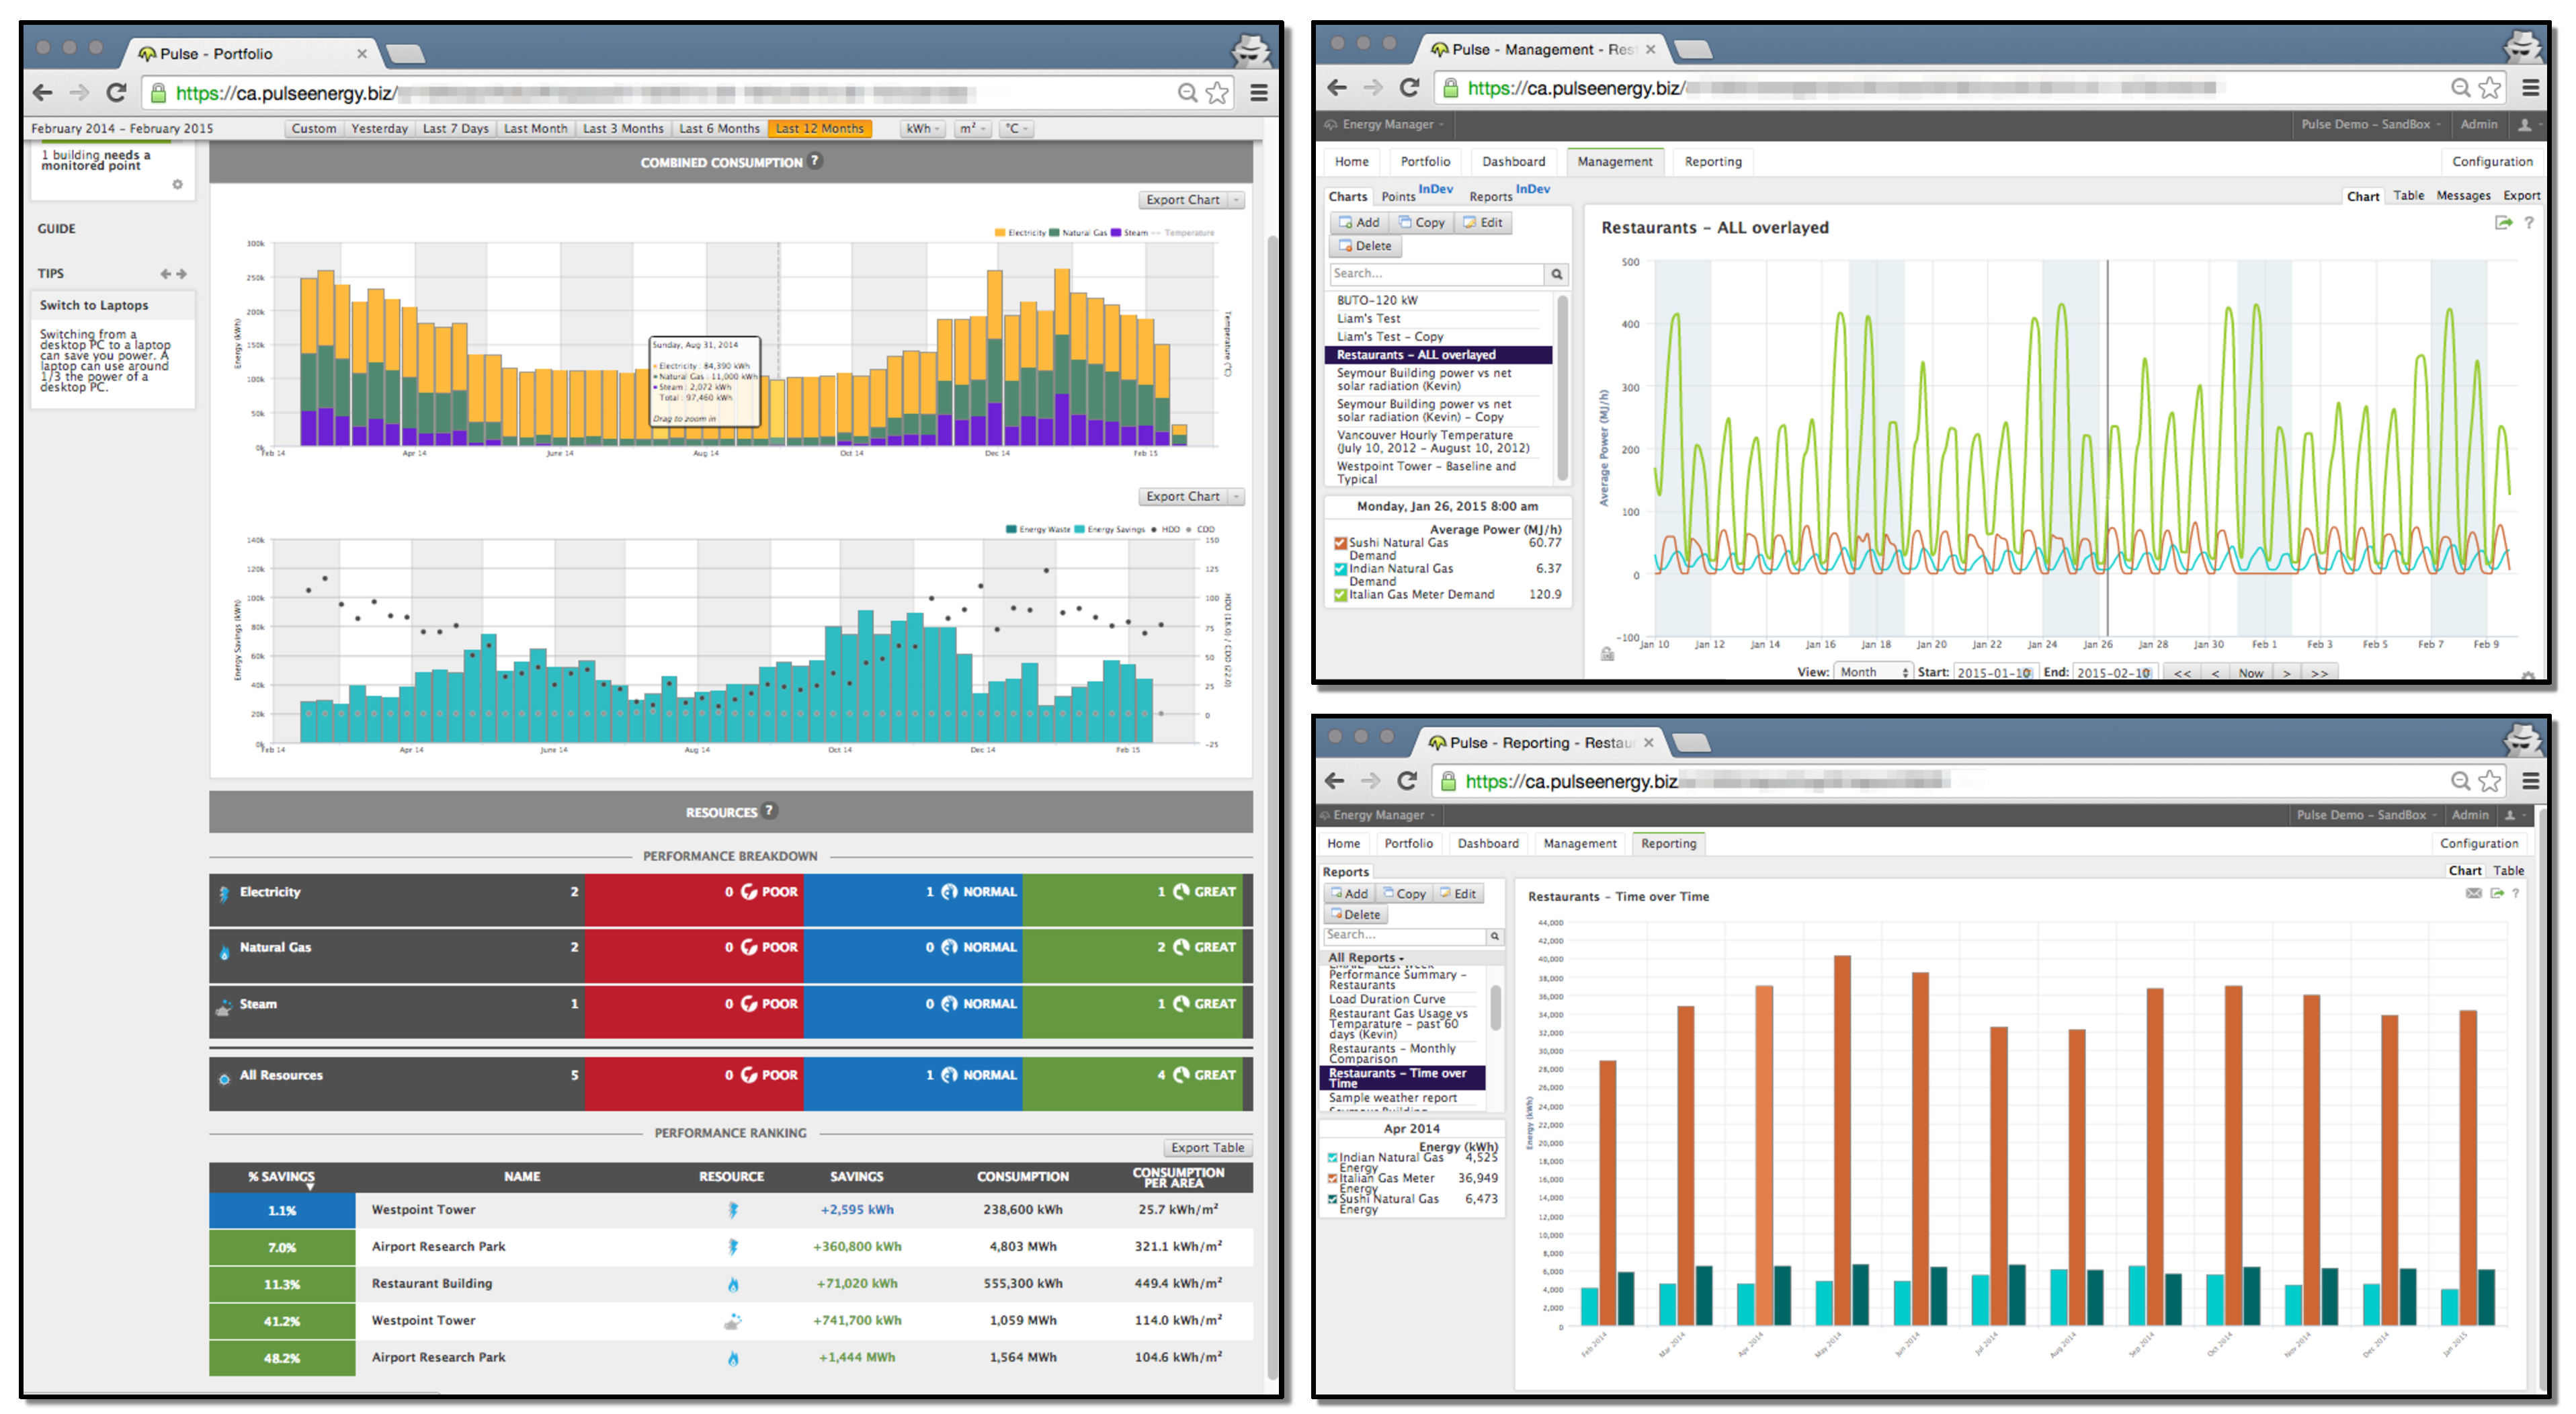
\includegraphics[width=\textwidth]{figures/em.pdf}
	\vspace{-0.6cm}
	\caption{\textsl{Energy Manager}, our collaborators' existing energy analysis tool. (a) A dashboard for a portfolio of buildings. (b) A superimposed line chart of \textsl{energy demand} and (c) a grouped bar chart of \textsl{energy consumption} (bottom) for a group of three restaurant buildings within this portfolio.}
	\label{fig:energy-manager}
% 	\vspace{-0.6cm}
\end{figure*} 

Energy workers need to balance reducing costs and conserving energy while ensuring the comfort and safety of people who use buildings in their portfolio. % \jn{edit for saying need 2 times here}
To achieve these goals, the energy workers need to: ({\bf i}) assess the performance of buildings in their portfolio following the implementation of an energy conservation measure, such as installing new windows or lighting; ({\bf ii}) determine which buildings in their portfolio require energy conservation measures; and ({\bf iii}) find and diagnose anomalous energy performance such as spikes, outages, surges, or otherwise erratic and inconsistent behaviour.

We characterize these activities as abstract tasks according to a typology that distinguishes between \underline{{\tt action}} and {\tt target} terms~\cite{Munzner2014}, one that builds upon a previous typology~\cite{Brehmer2013}; it can be helpful to think of {\tt actions} as verbs and {\tt targets} as nouns.
% These abstract tasks are summarized in Table~\ref{tab:task-abstractions}, and terms from this typology appear in a {\tt fixed-width font}.
Each of the tasks can be described by a need to \underline{{\tt discover}}: to generate and verify hypotheses.
While energy workers also occasionally \underline{{\tt present}} their findings to colleagues and other stakeholders, our current focus is predominantly on the discovery process. 

\bstart{T1 / Overview} An individual will \underline{{\tt lookup}} and \underline{{\tt summarize}} time-oriented data from all the items spanning a coarse period of time. 
Of interest are {\tt trends}, {\tt outliers}, {\tt distributions}, {\tt extreme values}, and {\tt similarities}. 
This abstract task corresponds to the domain activities of assessing overall energy performance and determining which buildings in a portfolio require energy conservation measures. 
A concrete example of this task would be an energy worker who asks: {\it ``how did the entire university perform this past year? Do any buildings stand out?''}
% A general question like this may also arise when {\tt presenting} findings.

\bstart{T2 / Drill Down} The second task is the result of drilling down from the portfolio to a group of buildings and to a finer temporal resolution, examining energy performance in detail: a person \underline{{\tt locates}} and \underline{{\tt compares}} {\tt trends}, {\tt outliers}, and {\tt features} in time-oriented data for items in the group.
This abstract task corresponds to the domain activities of assessing building performance following an energy conservation measure, or finding and diagnosing anomalous energy performance, wherein a {\tt feature} of interest could be a spike or sudden outage.
One concrete example is {\it ``are my restaurants in Vancouver performing better this January than they did last January?''}

\bstart{T3 / Roll Up} The third task is the converse of drilling down from the portfolio to a group and from the group to individual buildings.
This task is one in which a person \underline{{\tt explores}} and \underline{{\tt locates}} {\tt trends}, {\tt outliers}, and {\tt features} in time-oriented data to \underline{{\tt identify}} the proportion of individual behaviour relative to the group's behaviour, or the {\tt dependency} between the aggregate amount and the individual contribution.
Concrete examples of this task include {\it ``what proportion of a university's energy consumption is consumed by its computer science building over time?''} or {\it ``which science faculty building consumes the largest proportion of energy?''}

\bstart{Task sequences} These three tasks are not performed in isolation, but in sequential energy analysis workflows, and some task sequences occur more often than others. 
We know from our interviews that the frequency of this work varies, so the Overview ({\bf T1}) task may be more prevalent among energy workers who infrequently analyze their portfolio's energy performance.
Others may skip the Overview task because they have a specific question about a group of buildings, proceeding directly to the Drill Down ({\bf T2}) or Roll Up ({\bf T3}) tasks. 
An energy worker will alternate between the Drill Down and Roll Up tasks, as the completion of one task may prompt new questions.

%-------------------------------------------------------------------------
%-------------------------------------------------------------------------

\section{Existing Tool}
\label{existing-tool}

%-------------------------------------------------------------------------
%-------------------------------------------------------------------------

We now analyze the existing Energy Manager tool and determine the extent to which the tasks are supported.

% We focus on Energy Manager first, our collaborator's existing software, which all of the energy workers we interviewed had used to a varying extent for performing portfolio energy analysis.

Energy Manager, shown in Figure~\ref{fig:energy-manager}, is a multiple-page web-based application, one that uses a small number of visual idioms adhering to the domain convention mentioned in Section~\ref{abstractions}: bar charts and tables are used for derived aggregate values such as {\it consumption}, while line charts are used for continuous values such as {\it energy demand}.
The main page presents a summary dashboard for a portfolio of buildings (Fig.~\ref{fig:energy-manager}a). 
At the bottom of this dashboard is a sortable table listing {\it consumption}, {\it intensity}, as well as aggregate {\it savings} values for the currently selected time period. 

Line and bar charts such as those in Figures~\ref{fig:energy-manager}b and~\ref{fig:energy-manager}c are indexed on the other pages, similar to how a Microsoft Excel workbook has sheets, which can in turn contain multiple charts. 
Unlike Excel, Energy Manager's visualizations provide some interactivity: the user can zoom, pan, and reveal values upon mouseover. 
However, none of the visualizations are directly linked to one another or to the dashboard, so the energy worker must navigate between them manually.

\bstart{Task support} Energy Manager only partially supports the Overview ({\bf T1}) task: with the portfolio dashboard (Fig.~\ref{fig:energy-manager}a), the energy worker can observe the aggregate {\it consumption} for a portfolio over time, or alternatively she can observe single aggregate values for individual buildings in the sortable table, but she will not be able to directly compare how individual buildings vary over time.
As a result, the energy workers that we interviewed essentially ignored this dashboard, and none of them had found the sortable table to be useful. 
% \tm{too weak? earlier you said not at all. rephrase to 'essentially ignored'?...}

The Drill Down ({\bf T2}) task is supported but the current approach used by Energy Manager does not scale.
The examples in Figures~\ref{fig:energy-manager}b and~\ref{fig:energy-manager}c respectively display {\it energy demand} and {\it consumption} performance for three restaurants.
Since superimposed line charts and grouped bar charts are limited by the number of discriminable colours, these visualizations are inappropriate for the energy worker who needs to consider more than a handful of buildings.

The Roll Up ({\bf T3}) task is not explicitly supported. Though it is possible to estimate the proportion of a building's energy performance relative to its group with bars and lines, this process is error-prone.

\bstart{Task sequences not supported} Because the visualizations in Energy Manager are not coordinated or linked in any way, it is difficult and tedious to alternate from Overview ({\bf T1}) to Drill Down ({\bf T2}) and Roll Up ({\bf T3}) Tasks. 
As in Excel, the energy worker will have to locate an existing visualization or specify a new visualization using a wizard dialog; if the bar or line chart for a set of buildings does not already exist when the energy worker needs it, she has to create it. 
By the time she has created it, she may have forgotten her objective.

\bstart{Limited filtering and aggregation} The bar and line charts in Energy Manager allow an energy worker to hide or show individual buildings.
However, the energy worker cannot filter buildings with shared attributes, such as filtering a portfolio of buildings to only show restaurants.
Similarly, it is impossible to aggregate buildings together when they share attributes: for instance, the energy worker cannot compare the aggregate energy performance of restaurants in one city to those in another city.

\bstart{No faceting} Aside from the seldom-used portfolio dashboard shown in Figure~\ref{fig:energy-manager}a, there is no faceting or juxtaposition of visualizations in Energy Manager: the energy workers' workarounds included opening multiple browser windows, adjusting the line or bar charts to display the same scale and ranges, and tiling these windows manually across their monitor. 
Similarly, some energy workers printed and taped charts together to accomplish the same result.
% \jn{Printing out graphs on paper happened as well since limited screen space exacerbated the problem, I found this forced move from the software environment into an analog format a more alarming indication of this feature hole.}

\bstart{Summary} Due to these limitations, energy workers can only observe narrow slices of their portfolio data, or they are presented with aggregate data that is too coarse to be useful.
In addition, they did not trust Energy Manager's derived predicted values based on statistical models, and would have preferred to compare observed energy performance to historical values.
In other words, the derived and aggregated values currently shown may hide information such as extreme values and unusual distributions.
As a result of this loss of detail, energy workers routinely export tabular data from Energy Manager and import it into Excel, with which they would conduct a custom analysis.
Finally, many of the energy workers to whom we spoke remarked that energy analysis software tools built by our collaborators' competitors~\cite{Energent,Northwrite,Schneider}~have limitations similar to those of Energy Manager.
Altogether, these problems may help to explain why the number of energy workers who actively use Energy Manager is substantially less than the number of user accounts.

%-------------------------------------------------------------------------
%-------------------------------------------------------------------------

\section{Related Work}
\label{related-work}

%-------------------------------------------------------------------------
%-------------------------------------------------------------------------

We now review relevant previous work, beginning with work in the energy domain. 
We also discuss visualizations of time-oriented data in other domains, as well as evaluation studies that assess the effectiveness of visualization idioms for similar data and task abstractions.

\bstart{Visualization in the energy domain} Technology that allows for the continuous measurement of a building's energy demand is becoming increasingly available, and several techniques to monitor and present this data have recently been proposed, especially for residential buildings~\cite{Ellegard2011,Erickson2013,Goodwin2013,Rodgers2011}.
Erickson~\etal~\cite{Erickson2013} developed a web-based residential energy dashboard for homeowners, allowing them to compare against their neighbours with familiar bar and line charts.
However, such a dashboard would be unsuitable for the analysis work of an energy worker who oversees a portfolio of many buildings.

Though bar and line chart depictions of energy data are most common, other visual encodings have also been employed, from abstract and artistic ambient visualizations~\cite{Rodgers2011} to a compelling calendar-based visualization~\cite{vanWijk1999}, in which calendar dates with similar energy behaviour are visually associated using a common colour.
We also explore visual encodings beyond bar and line charts, and in Section~\ref{design-matrix}, we consider how to encode data from multiple buildings using calendars.
Another approach to summarizing the energy behaviour of multiple buildings is to use map-based visualizations~\cite{Heat2014,MEP2014}; we discuss the limitations of that approach in Section~\ref{design-map}. 

More closely related to our work is that of Goodwin~\etal~\cite{Goodwin2013}, who presented several prototype visualizations of modelled residential energy use across thousands of households at the scale of individual household appliances. 
The domain activities they address overlap partially with those performed by the energy workers we spoke to, such as the need to find anomalous energy performance across many buildings; another activity they address, in which energy modelers perform energy load-shifting simulations to estimate potential savings, is not an activity performed by our energy workers. 
Their designs incorporated several visual encodings not typically seen in the energy domain: horizon charts~\cite{Heer2009}, boxplots~\cite{Wickham2011}, and matrix-based encodings.
However, the focus and main contribution of their paper was on creative methods for visualization requirements analysis, rather than on a thorough analysis of the visualization designs themselves.
In our work, we reexamine some of these visual encodings, among others, and evaluate their effectiveness in the context of our data and task abstractions. 

\bstart{Visualizing multiple time series} Many techniques for visualizing time-oriented data have been proposed, and Aigner~\etal's 2011 survey~\cite{Aigner2011} of these visualizations has provided us with a structured way to think about this design space.
% Many of these visualizations are domain-agnostic, while others were developed in the context of a particular domain. 
In their terminology, our designs incorporate {\it linear} and {\it cyclic} encodings of time, depicting {\it abstract multivariate interval} data.

Another axis on which we can analyze existing techniques is the number of time series being considered.
At the low end of this continuum, superimposed line charts or grouped bar charts are appropriate for a small number of time series. 
% ; since these typically use colour to differentiate items, these techniques tend to be effective for less than a dozen time series~\cite{Munzner2014}.
In the middle of this continuum, faceting techniques such as small multiple line charts, horizon charts~\cite{Heer2009} and matrix-based encodings~\cite{Hao2007,Shimabukuro2004} are appropriate.
At the high end of this continuum, dense multi-form faceting techniques and those that aggregate time series together are appropriate when dealing with thousands of time series, such as in LiveRAC~\cite{McLachlan2008} or Line Graph Explorer~\cite{Lam2007}. 
Since we are addressing portfolios of dozens to hundreds of buildings, we position our designs toward the middle of this continuum, and we evaluate faceting and matrix-based approaches in the following section.
% we do not consider horizon charts since they are intended for continuous time series

\begin{figure*}[ht]
    % \vspace{-0.3cm}
	\centering
	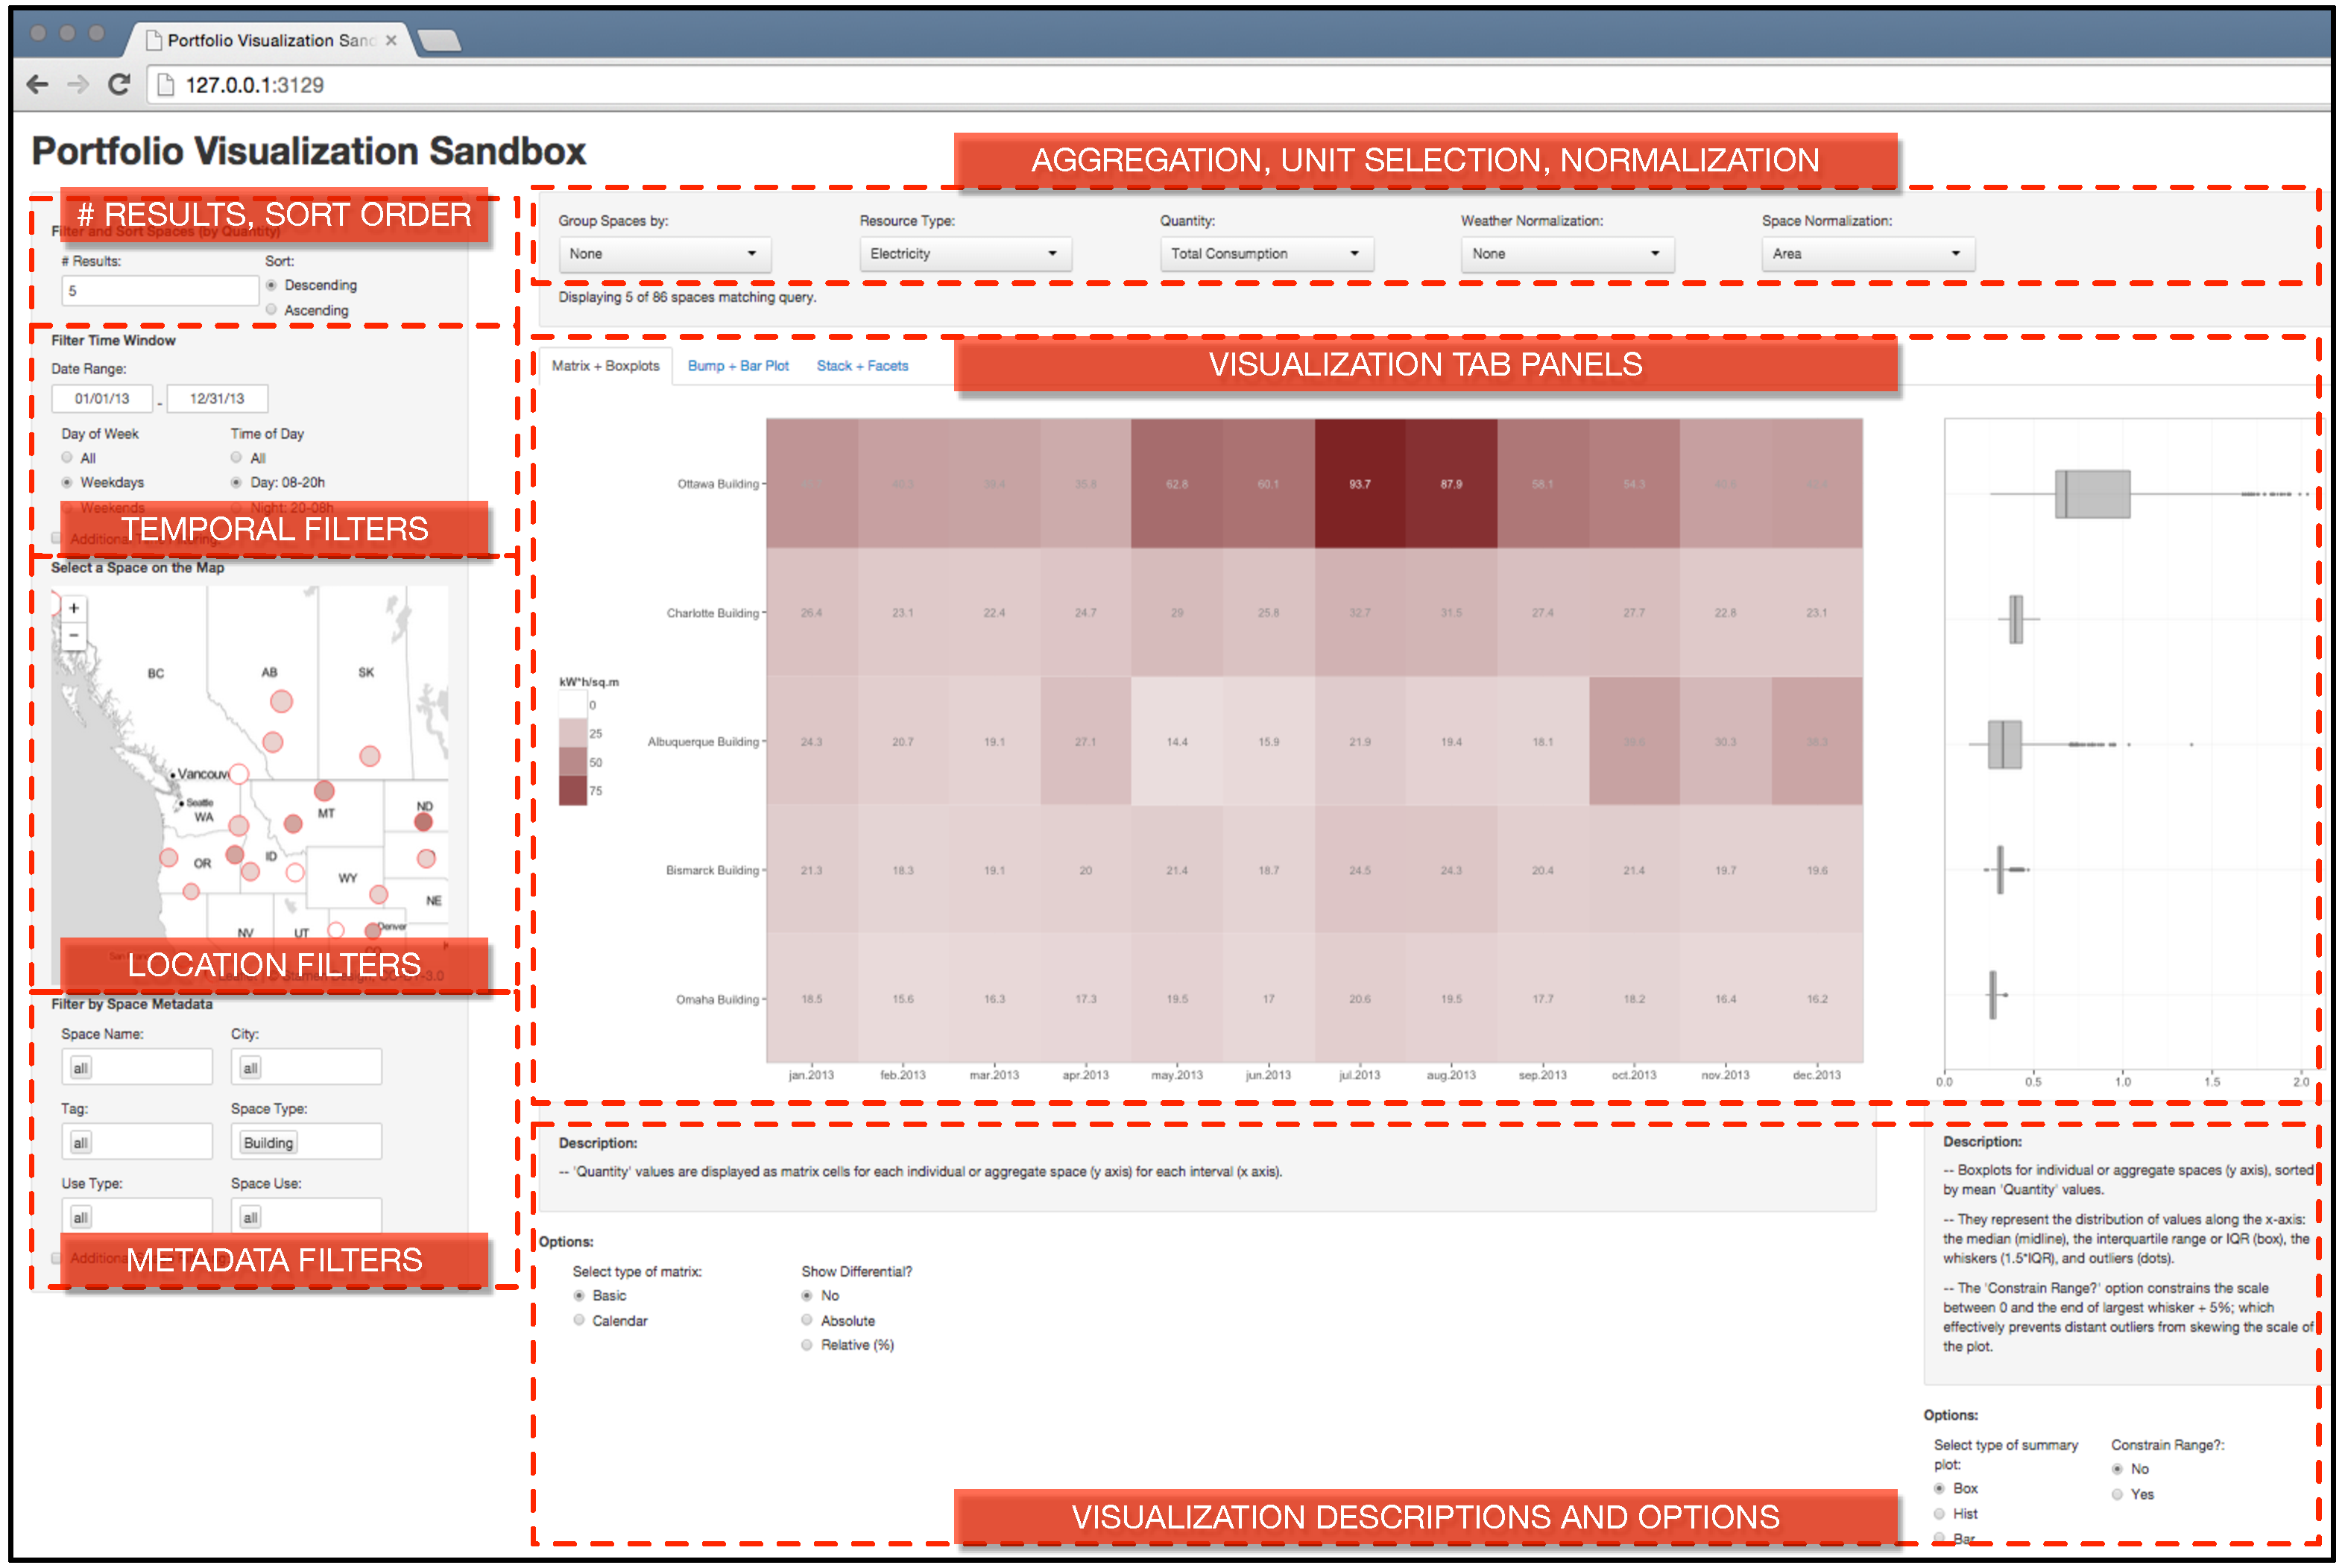
\includegraphics[width=\textwidth]{figures/sandbox.pdf}
	\vspace{-0.6cm}
	\caption{A sandbox design environment for visualizing energy data from a portfolio of buildings. Designs depicted in Figures~\ref{fig:sandbox-faceted-boxplot},~\ref{fig:sandbox-barbump},~\ref{fig:sandbox-calendar}, and~\ref{fig:sandbox-stacks} were also produced within this environment. A matrix of aggregate \textsl{energy intensity} values with auxiliary boxplots is shown for 5 (of 86) buildings, those with the highest \textsl{intensity}.
	Client portfolio data has been anonymized by changing building names and location; all other data is real.}
	\label{fig:sandbox}
	\vspace{-0.45cm}
\end{figure*} 

\bstart{Evaluation of time-oriented data visualizations} We also situate our work with regards to experimental studies~\cite{Albers2014,Correll2012,Fuchs2013,Javed2010} that have examined the viability of alternative visual encodings for abstract tasks similar to those that we characterized: identifying and comparing averages, trends, extreme values, and outliers.
Some studies address the viability of encodings for a single time series~\cite{Albers2014,Correll2012}, while others consider multiple concurrent time series; one study considered up to sixteen time series~\cite{Javed2010}, while another considered forty-eight~\cite{Fuchs2013}.
We too assessed the viability of different visual encodings for multiple concurrent time series; however, our approach involves a qualitative evaluation (see Section~\ref{methodology}), as opposed to a controlled experiment.

% Albers~\etal~\cite{Albers2014} compared eight visual encodings of a single continuous time series for tasks in which the viewer is asked to identify one of seven aggregate values, such as the minima, maxima, average, or number of outliers. 
% They do not examine the effectiveness of these encodings in faceted visualizations of multiple time series, which we address in the following section.%; specifically, we consider faceted line charts and boxplots.
% % We also examined colour stock charts, though our findings were inconclusive.

% As for multiple time series, Javed~\etal~\cite{Javed2010} compared the effectiveness of two superimposed encodings (a line chart and a braided graph) to two faceted encodings (small multiple line charts and horizon graphs) for data containing up to 16 concurrent time series.
% Since our energy workers need to consider dozens to hundreds of concurrent time series, we are skeptical that their findings generalize to our situation, and we discuss alternative encodings in the following section. 
% % Finally, Fuchs~\etal~\cite{Fuchs2013} evaluated four alternative faceted encodings for 48 concurrent time series.

Moreover, while these studies considered continuous time series data, we must consider alternative scalable encodings, since in our case domain conventions dictate that continuous line graph encodings would be misleading for the display of derived and aggregated time series values, as discussed in Section~\ref{data-abstractions}.
% \tm{This point isn't clear enough - why exactly?! Is it just that they have a domain convention that line chart equals raw data, or something else more subtle?}

%-------------------------------------------------------------------------
%-------------------------------------------------------------------------

\section{Prototyping Environments}
\label{sandbox}

%-------------------------------------------------------------------------
%-------------------------------------------------------------------------

\bstart{Shiny sandbox}
We developed an interactive browser-based visualization design sandbox\footnote{\small{\url{http://mattbrehmer.shinyapps.io/PortfolioSandbox}}} to produce {\it data sketches}~\cite{Lloyd2011}, shown in Figure~\ref{fig:sandbox}. 
The sandbox allowed us to rapidly prototype different visual encoding designs and conduct chauffeured workflows with energy workers, a process that we described in Section~\ref{methodology}. 
All of the designs discussed in Section~\ref{design:visenc} were produced within this environment, which was developed\footnote{\small{\url{http://github.com/mattbrehmer/PortfolioSandbox}}} using the Shiny web application framework~\cite{shiny}.

Central to this sandbox environment are interactive controls for sorting, filtering, and aggregating buildings, controls for selecting units of interest such as {\it demand} or {\it consumption}, as well as controls for area and weather normalization; recall that there were no such controls in the Energy Manager interface.
Whenever these controls are adjusted, we sort the filtered set of buildings according to the currently selected energy unit of interest and time span.
The sandbox operator can choose the sort order and select the number of results to show. 
For instance, Figure~\ref{fig:sandbox} shows a view described in Section~\ref{design-matrix}, and in it we show 5 buildings from a geographically anonymized portfolio of 86 buildings, those with the highest {\it energy intensity} in 2013. 
% We deployed this visualization sandbox environment on our collaborator's local intranet. 
% It is also accessible publicly, though we had to use a small anonymized dataset for the latter due to client privacy concerns.

\bstart{D3 interactive prototypes}
Since our Shiny-based sandbox implementation did not allow us to directly experiment with interactions involving coordinated selection across juxtaposed views, we developed several interactive prototypes using D3~\cite{Bostock2011} that specifically address this coordination;  these prototypes are discussed in Section~\ref{design:workflows} and one of them \footnote{\small{\url{http://bl.ocks.org/mattbrehmer/287e44c9a12151967874}}} is shown in Figure~\ref{fig:interactive-boxplots}.

%-------------------------------------------------------------------------
%-------------------------------------------------------------------------

\section{Visual Encoding Matches and Mismatches}
\label{design:visenc}

%-------------------------------------------------------------------------
%-------------------------------------------------------------------------

The Nested Blocks and Guidelines Model~\cite{Meyer2013} describes a need for guidelines that relate the domain, abstraction, idiom (technique), and algorithm levels of visualization design~\cite{Munzner2009,Munzner2014}.
In Section~\ref{abstractions}, we described the relationship between domain activities and the data and task abstractions.
In this section, we consider the space of visual encoding idioms and present guidelines for matching idioms to abstractions. 
Since the space of possible visual encoding idioms for time-oriented data is large~\cite{Aigner2011}, we undertook a typical design study approach~\cite{Sedlmair2012}: considering several idioms, implementing a subset of them, and selecting only the few good matches.
% based on an evaluation that was conducted alongside of our design process. 
% \tm{concided with sounds a little odd - you mean 'was conducted within'?...}

We identified five {\it matches} \{\match\} between visual encoding idioms and the combination of data and task abstractions, based on evidence resulting from our process described in Section~\ref{methodology}. 
We also identified four {\it mismatches} \{\mismatch\} and two {\it potential matches} \{\posmatch\}. 
These matches and mismatches, summarized in Table~\ref{tab:matches-mismatches}, serve as generalizable guidelines that are transferable beyond the energy domain, especially when we consider the similarity between our abstract tasks to those addressed in domain-agnostic evaluation studies~\cite{Albers2014,Javed2010}.
Furthermore, these matches and mismatches fill a gap with regards to identifying suitable visual encoding idioms for multiple time series in which values are not continuous, but derived and aggregated values that should {\it not} be encoded as line charts.
% Evidence for these matches and mismatches emanates from an evaluation that was conducted alongside our design process, which involved both our collaborators and external energy workers.
% We now present a subset of the findings from these sessions for each of the visualizations that we considered.

\begin{table}[ht]\renewcommand{\arraystretch}{1.2}\addtolength{\tabcolsep}{-1pt}
    \vspace{-.15cm}
    \begin{center}
    \scriptsize
    \begin{tabular}{l|l|c}

        \rowcolor{blue!15}
    
        {\bf Task} & {\bf Visualization Idiom} & {\bf Match?}
        
        \\
        
        %task
        {\bf T1}: Overview 
        
        %idiom
        & Faceted bar chart 
        
        %match?
        & \mismatch
        
        \\
        
        \rowcolor{gray!15}
        
        %task
        %{\bf T1}: Overview 
        
        %idiom
        & Bump plot 
        
        %match?
        & \mismatch
        
        \\
        
        %task
        %{\bf T1}: Overview 
        
        %idiom
        & Bar + bump plot 
        
        %match?
        & \posmatch
        
        \\
        
        \rowcolor{gray!15}

        %task
        %{\bf T1}: Overview 
        
        %idiom
        & (Calendar) matrix 
        
        %match?
        & \posmatch
        
        \\
        
        %task
        %{\bf T1}: Overview 
        
        %idiom
        & Map 
        
        %match?
        & \mismatch
        
        \\
        
        \rowcolor{gray!15}
        
        %task
        %{\bf T1}: Overview 
        
        %idiom
        & Juxtaposed matrix and boxplots 
        
        %match?
        & \match
        
        \\
        
        
        \hline
        
        %task
        
        {\bf T2}: Drill Down 
        
        %idiom
        & Faceted bar chart 
        
        %match?
        & \match
        
        \\
        
        \rowcolor{gray!15}
        
        %task
        %{\bf T2}: Drill Down 
        
        %idiom
        & Faceted boxplot 
        
        %match?
        & \mismatch
        
        \\
        
        %task
        %{\bf T2}: Drill Down 
        
        %idiom
        & Faceted line graph 
        
        %match?
        & \match
        
        \\
        
        \rowcolor{gray!15}
        
        \hline
        
        %task
        {\bf T3}: Roll Up 
        
        %idiom
        & Stacked area graph 
        
        %match?
        & \match
        
        \\
        
        %task
        %{\bf T3}: Roll Up 
        
        %idiom
        & Stacked bar chart 
        
        %match?
        & \match
        
        \\
        
        \hline  
        
    \end{tabular}
    \vspace{-0.15cm}
    \caption{A summary of the \textsl{matches} and \textsl{mismatches} between abstract tasks and visual encoding idioms.}
    \label{tab:matches-mismatches}
    \end{center}
    \vspace{-0.6cm}
\end{table}

%-------------------------------------------------------------------------

\subsection{Faceted Visualizations for Overview and Drill Down}
\label{design-faceting}

%-------------------------------------------------------------------------'

We initially thought that faceted ``small multiple'' visualizations would be a good match for {\it both} the Overview ({\bf T1}) and Drill Down ({\bf T2}) tasks, in that they provide a scalable alternative to grouped bar charts and superimposed line charts.

\bstart{Faceted bar charts} {\it a mismatch} \{\mismatch\} {\it for the} Overview ({\bf T1}) {\it task, yet a match} \{\match\} {\it for the} Drill Down ({\bf T2}) {\it task}.
Faceted bar charts were among the first designs that we considered, especially after one energy worker provided us with his own mockup of such a design.
However, if an energy worker has dozens or hundreds of buildings in their portfolio, faceting is unlikely to scale~\cite{Javed2010}. 
We determined that it was a poor match for the Overview ({\bf T1}) task, though a match for the Drill Down ({\bf T2}) task, provided that the energy worker has already filtered down to a smaller group of buildings, such as filtering a university portfolio to show only the {\it ``laboratory''} buildings.
In addition, one of the power user energy workers lamented that bar charts only show coarse aggregate values, typically an average or a sum, and as a result of this loss of detail, they do not show other aggregate values of interest, such as ranges or extreme values.

\bstart{Faceted boxplots} {\it a mismatch} \{\mismatch\} {\it for the} Drill Down ({\bf T2}) {\it task}.
We expected that faceted boxplots would allow energy workers to compare ranges, distributions, and extreme values for multiple buildings at different points in time, such as in Figure~\ref{fig:sandbox-faceted-boxplot}.
However, despite the long history of boxplots~\cite{Wickham2011} and support from influential visualization practitioners~\cite{Few2014}, we found that most energy workers are not familiar with boxplots, except for a minority who had taken a post-secondary statistics course.
Furthermore, comparisons in faceted boxplots are more difficult than in faceted bar charts, where positions are aligned to each facet's baseline; with faceted boxplots, the observer must compare multiple positions and widths across separate facets. 
Our design was therefore a daunting introduction to boxplots for those unfamiliar with them and a poor match for the Drill Down task.

\begin{figure}[ht]
    \vspace{-0.3cm}
	\centering
	\fbox{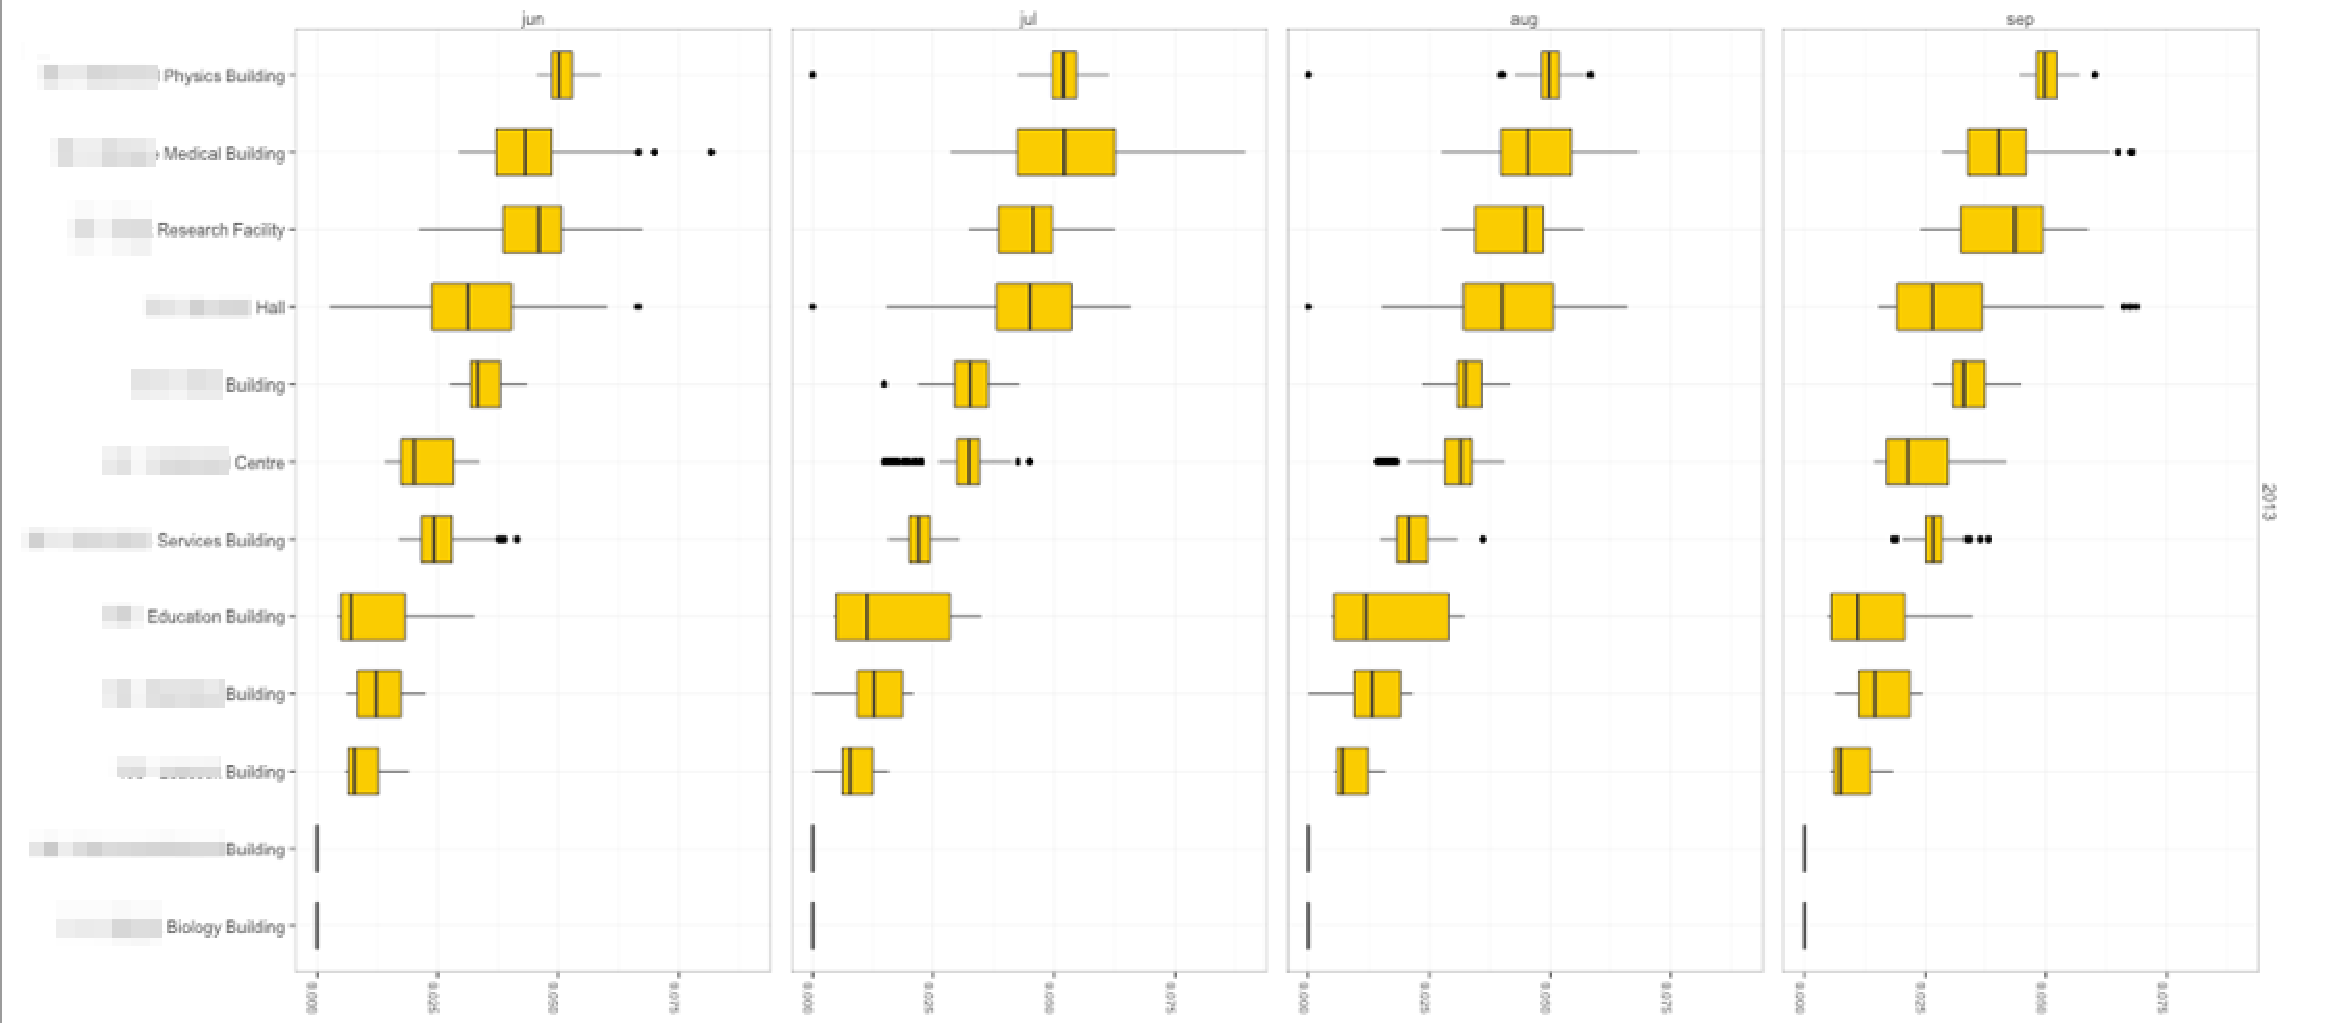
\includegraphics[width=0.95\columnwidth]{figures/sandbox-faceted-boxplot.pdf}}
	\vspace{-0.15cm}
	\caption{Faceted boxplots that encode aggregate area-normalized energy \textsl{demand} distributions for 12 buildings across four months, sorted in descending order according to the average \textsl{demand} value for this four month period. A mismatch  \{\mismatch\} for the Drill Down task (T2). Building names are blurred to sanitize real client portfolio data.}
	\label{fig:sandbox-faceted-boxplot}
	\vspace{-0.3cm}
\end{figure} 

\bstart{Faceted line charts} {\it a match} \{\match\} {\it for the} Drill Down ({\bf T2}) {\it task}.
Faceted line charts are a good match when observing non-derived continuous quantitative time series values such as {\it energy demand}; an example is shown in Figure~\ref{fig:sandbox-stacks} (bottom).
They are a scalable alternative to superimposed line charts~\cite{Javed2010} and the line chart encoding is already very familiar to energy workers.
As mentioned above in Section~\ref{abstractions}, line charts are {\it not} appropriate for derived and aggregated values such as {\it energy consumption} or {\it intensity}.

%-------------------------------------------------------------------------

\subsection{Rank-Based Overview Visualizations}
\label{design-ranking}

%-------------------------------------------------------------------------

As faceting seemed unlikely to be effective for the Overview ({\bf T1}) task, we considered non-faceted visualizations of aggregate values.
Recall how the sortable table in Energy Manager's portfolio dashboard (Figure~\ref{fig:energy-manager}a, bottom) was never used for the Overview task; it contained only coarse aggregate values for each item, providing little detail about temporal variation.
We therefore experimented with encodings for displaying rank as well as rank change over time.

\bstart{Bump plots} {\it a mismatch} \{\mismatch\} {\it for the} Overview ({\bf T1}) {\it task}.
Bump plots encode rank and rank change; they incorporate a familiar line encoding across equally-spaced temporal intervals~\cite{Tufte1990}. 
However, as with superimposed line charts, it becomes difficult to distinguish individual items using colour.
One possible solution is to highlight items that vary in rank, rather than requiring the observer to locate these items.
Another problem is that bump plots only show relative rank and rank change, whereas the absolute values that produce these ranks are not shown. 
As a result this a loss of detail, the bump plot is also a poor match for the Overview task.

\bstart{Bump + bar plots} {\it a potential match} \{\posmatch\} {\it for the} Overview ({\bf T1}) {\it task}.
We next considered an encoding that incorporates relative rank, rank change, and absolute value, by adding bars to each series in the bump plot, as shown in Figure~\ref{fig:sandbox-barbump}. 
This approach is similar to two recently proposed techniques that encode both relative rank and absolute value~\cite{Gratzl2013,Hur2013}. 
With this design, we still face the scalability problem associated with colour discriminability.
A combination of interaction and highlighting rank variation may facilitate this discriminability; in Figure~\ref{fig:sandbox-barbump}, rank variation is encoded using the alpha channel, so the pink series that varies considerably over time is most salient.

\begin{figure}[ht]
    \vspace{-0.3cm}
	\centering
	\fbox{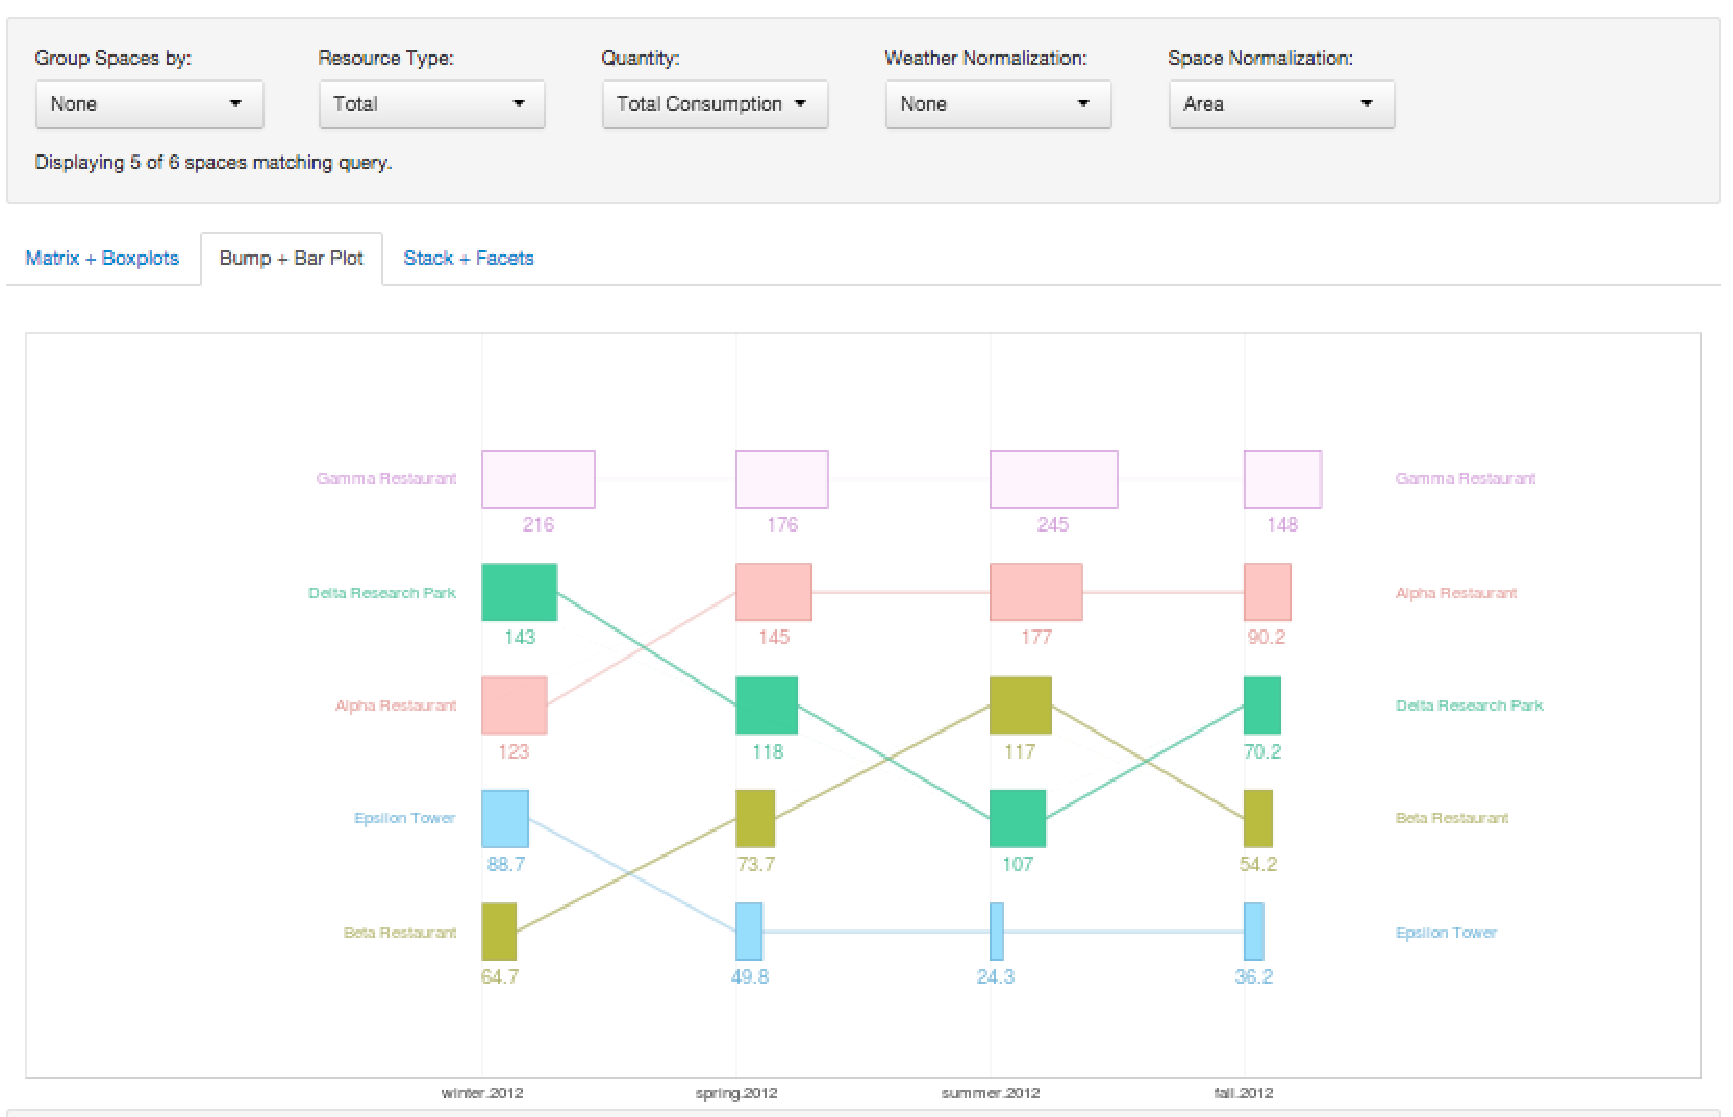
\includegraphics[width=0.95\columnwidth]{figures/sandbox-barbump.pdf}}
	\vspace{-0.15cm}
	\caption{A \textsl{bar + bump plot} of \textsl{energy intensity}, encoding rank change for the top 7 building groups (buildings aggregated by tag) across four seasons. The alpha channel encodes rank variation to highlight inconsistent buildings. A potential match  \{\posmatch\} for the Overview task (T1).}
	\label{fig:sandbox-barbump}
	\vspace{-0.3cm}
\end{figure}

Energy workers responded positively to this visualization, as it is comprised of familiar bar and line encodings. 
However, despite this positive response, we discovered that {\it ranks} as derived values are actually infrequently considered during energy analysis, and that they tend to be more appropriate for annual planning and presentation activities, such as determining how to prioritize energy conservation projects, and less so for recurring analysis and monitoring activities.
% at the beginning of energy conservation projects or when energy workers {\it present} their findings to colleagues on a quarterly or annual basis. 
% \jn{also used infrequently at the beginning of planning stage(one yearly) to prioritize buildings that will get EC projects.  Out of a large portfolio and with energy manager's time a limited resource, ranking was used as a quick way to just choose which buildings will receive the most attention for the year.}
Thus, the hunt for a match for the Overview ({\bf T1}) task continued.
% We also identified four {\it mismatches} and one potential match: that of the {\it bump + bar plot} described in Section~\ref{design-ranking}; our hesitation to call this a match stems not from a problem with the visualization itself, but from energy workers' low priority on ranks as derived data of interest.

%-------------------------------------------------------------------------

\subsection{Matrix-Based Overview Visualizations}
\label{design-matrix}

%-------------------------------------------------------------------------

\bstart{Time series matrix} {\it a potential match} \{\posmatch\} {\it for the} Overview ({\bf T1}) {\it task}.
Matrix encodings are scalable and space-efficient~\cite{Goodwin2013,Hao2007}, as can be seen in the center of Figure~\ref{fig:sandbox}.
Matrix encodings allow us to display observed as well as differential values, allowing an energy worker to review {\it energy savings} relative to predicted or historical values; a matrix displaying differential energy data is shown in Figure~\ref{fig:sandbox-calendar}. 
Most of the energy workers that we interviewed were unfamiliar with this form of encoding, except one who routinely made such visualizations in Excel. 
As a result, it took more effort to convince our collaborators of the value of these matrix-based encodings for the Overview task.

We also learned that energy workers found matrices with diverging colour scales easier to interpret than than those with unidirectional colour scales. 
Finally, we found that while red is fine for use in diverging colour scales, as it has a negative connotation, it is inappropriate for unidirectional colour scales in this context. 
As a result of this mixed response to matrix-based encodings, we realized that more work needed to be done.

\bstart{Calendar matrix} {\it a potential match} \{\posmatch\} {\it for the} Overview ({\bf T1}) {\it task}.
We altered our matrix encoding by partitioning the cells corresponding to months into calendars (Figure~\ref{fig:sandbox-calendar}), a design decision inspired by previous work~\cite{Lammarsch2009,vanWijk1999}. 
Energy workers responded positively to this encoding, which helped to resolve the unfamiliarity of the more generic matrix encoding. 
However, months and days are not the only time granularities of interest, so this encoding may not be appropriate for all time ranges.

\begin{figure}[ht]
    % \vspace{-0.3cm}
	\centering
	\fbox{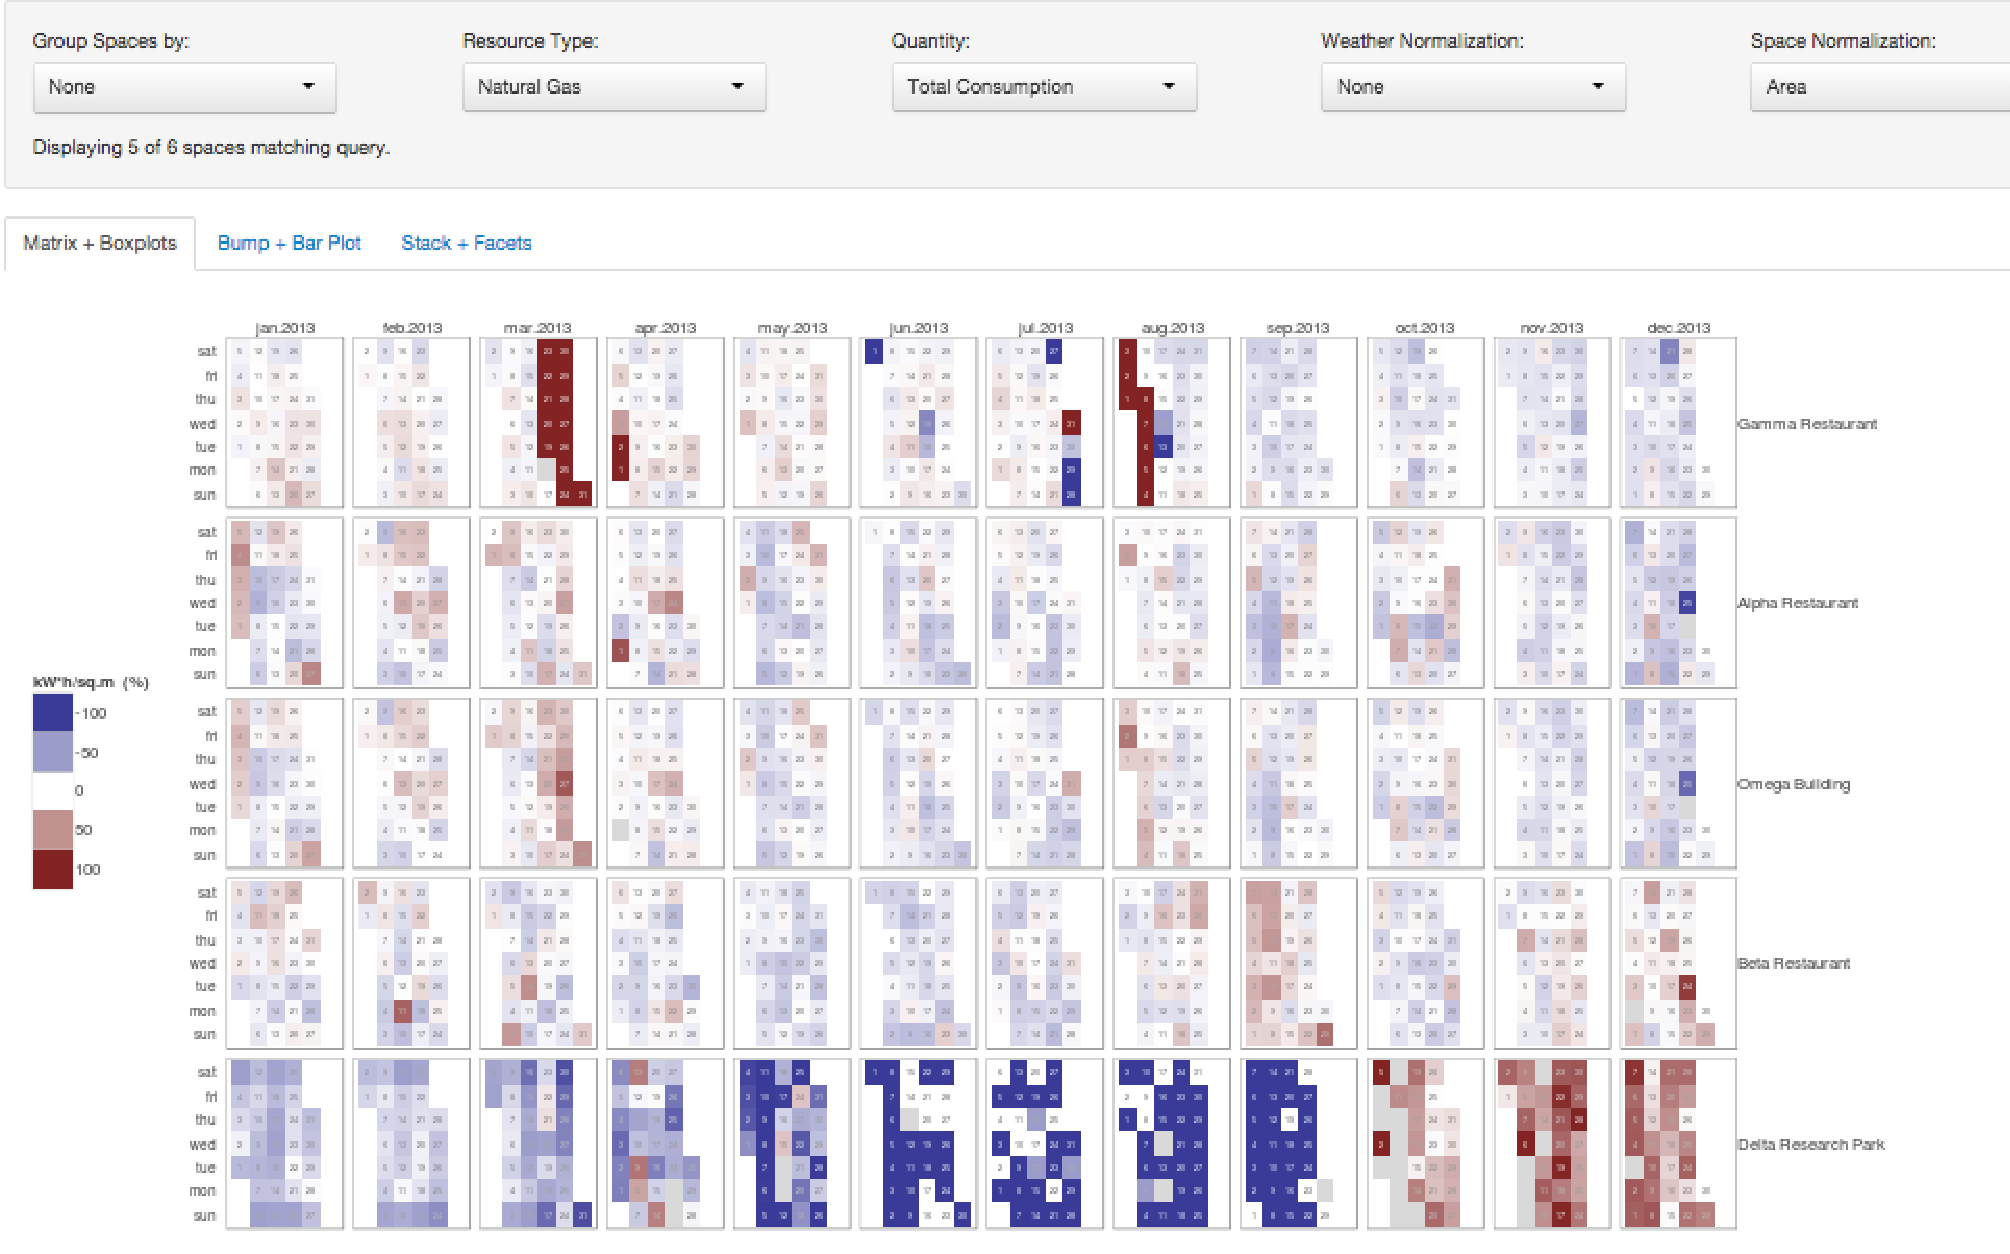
\includegraphics[width=0.95\columnwidth]{figures/sandbox-calendar.pdf}}
	\vspace{-0.15cm}
	\caption{A time series calendar matrix of \textsl{energy intensity savings} for 7 building groups (buildings aggregated by shared categorical tag), relative to historical values (blue = \textsl{savings}, red = higher than historical \textsl{intensity}). A potential match \{\posmatch\} for the Overview task (T1).}
	\label{fig:sandbox-calendar}
	\vspace{-0.6cm}
\end{figure}

%-------------------------------------------------------------------------

\subsection{Map-Based Overview Visualizations}
\label{design-map}

\bstart{Maps} {\it a mismatch} \{\mismatch\} {\it for the} Overview ({\bf T1}) {\it task}.
We explored the use of maps based on their popularity in previous work~\cite{Heat2014,MEP2014}. 
We conjectured that maps may be appropriate for buildings in a shared neighbourhood, such as a university campus, even though that encoding may be less appropriate for building portfolios spanning large geographic areas. 
However, after interviews with energy workers, we realized that maps are better suited for presenting coarse aggregate summary values of energy performance to a casual observer, and they are less appropriate for recurring analysis work; to view energy behaviour varying over time, animating or faceting the map would be necessary. 
Furthermore, an energy worker overseeing a portfolio of buildings is already likely to be familiar with the locations of buildings in her portfolio, and their relative locations are not informative. 
While using a map to encode energy data was found to be inappropriate for the tasks that we characterized, an interactive map may be an effective means to filter a portfolio by building location, which we considered in our sandbox environment shown in Figure~\ref{fig:sandbox}.

\subsection{Stack-Based Roll Up Visualizations}
\label{design-rollup}

%-------------------------------------------------------------------------

\bstart{Stacked area charts \& stacked bar charts} {\it matches} \{\match\} {\it for the} Roll Up ({\bf T3}) {\it task}.
The obvious visualizations of stacked area~\cite{Byron2008} and stacked bar charts were indeed matches; an example of the former is shown in Figure~\ref{fig:sandbox-stacks} (top).
Stacked area charts are appropriate when considering {\it energy demand} values, while stacked bar charts are appropriate for derived and aggregated values such as {\it energy consumption} or {\it intensity}.
For both of these encodings, differentiating individual time series can be accomplished by interactive highlighting~\cite{Wattenberg2005}, as using hue to differentiate stack elements will not scale.

%---------------------------------------------------------------------------

% \subsection{Summary of Matches and Mismatches} 
% \label{design-summary}

% %-------------------------------------------------------------------------

% We identified four {\it matches} between abstract tasks ({\bf T1--T3}) and visualization idioms. 
% Matches and mismatches are summarized in Table~\ref{tab:matches-mismatches}.

%-------------------------------------------------------------------------
%-------------------------------------------------------------------------

\section{Workflow Design with Multiple Views}
\label{design:workflows}

%-------------------------------------------------------------------------
%-------------------------------------------------------------------------

Our design discussion up to this point has focused on visual encoding choices for single views; we also want to stress the importance of interaction and workflow design, which involves juxtaposing and linking multiple views.
% Our sandbox environment allowed us to easily explore the design space of visual encodings, as well as interactions relating to the parametrization of a single view: filtering, aggregation, and deriving normalized values.
% However, the sandbox did not allow us to directly investigate interactions involving coordinated selection across juxtaposed views, nor did it allow us to easily prototype interactive workflows to support the task sequence from Overview ({\bf T1}) to Drill Down ({\bf T2}) and Roll Up ({\bf T3}).
% we also used it as a tool to generate storyboards of possible {\it workflows} that support a sequence of tasks, 

\bstart{Juxtaposed matrix and boxplots} {\it a match} \{\match\} {\it for the} Overview ({\bf T1}) {\it task}.
One reason to juxtapose views is to support a single task with complementary data.
None of the encodings discussed thus far are a clear match for the Overview task, although the time series matrix designs described in Section~\ref{design-matrix} showed promise.
A problem with the matrix encodings is that they display coarse aggregate values only, such as averages or sums for each matrix cell. 
Recall from Section~\ref{design-faceting} that an energy worker made the same remark about faceted bar charts.
Partitioning a matrix into calendars is one way to show a finer resolution in the same amount of space, however this encoding will not always be appropriate: for instance, an energy worker may be interested in a time span shorter than a month, or longer than several years.
The alternative that we developed involves complementing and reinforcing the aggregate values in the original matrix design by juxtaposing single boxplots that encode ranges and distributions for each time series, as shown in Figure~\ref{fig:sandbox}.
Though boxplots remain unfamiliar to energy workers, these auxiliary boxplots are easier to interpret than faceted boxplots (c.f. Figure~\ref{fig:sandbox-faceted-boxplot}), as they require no comparison of length or width across separate facets. 
We reflect further upon the balance between familiarity and the use of auxiliary charts to combat information loss in Section~\ref{discussion-guidelines}.

We then sought a better way to coordinate and link the matrix and its juxtaposed auxiliary boxplots. We created several prototypes, and one is shown in Figure~\ref{fig:interactive-boxplots}.
The interactive linked highlighting in this prototype served both to promote engagement with these juxtaposed visualizations and to facilitate the learning of these visual encodings, which were previously unfamiliar to energy workers.
% As a result, our collaborators agreed that this coordinated and juxtaposed design is a match \{\match\} for the Overview ({\bf T1}) task.
% \jn{also to connect the different time scales of the 2 visualizations together, which was a stumbling block found in user testing. The averaged values in the tiles represent different time periods, to the 15 min (?) interval data values from which the average is calculated, maybe this point is already covered by "facilitate learning" This comment is also worded horribly, sorry.}
% These prototypes further convinced our collaborators that a time series matrix with juxtaposed auxiliary boxplots was a good match for the Overview ({\bf T1}) task.

\begin{figure}[ht]
    \vspace{-0.3cm}
	\centering
	\fbox{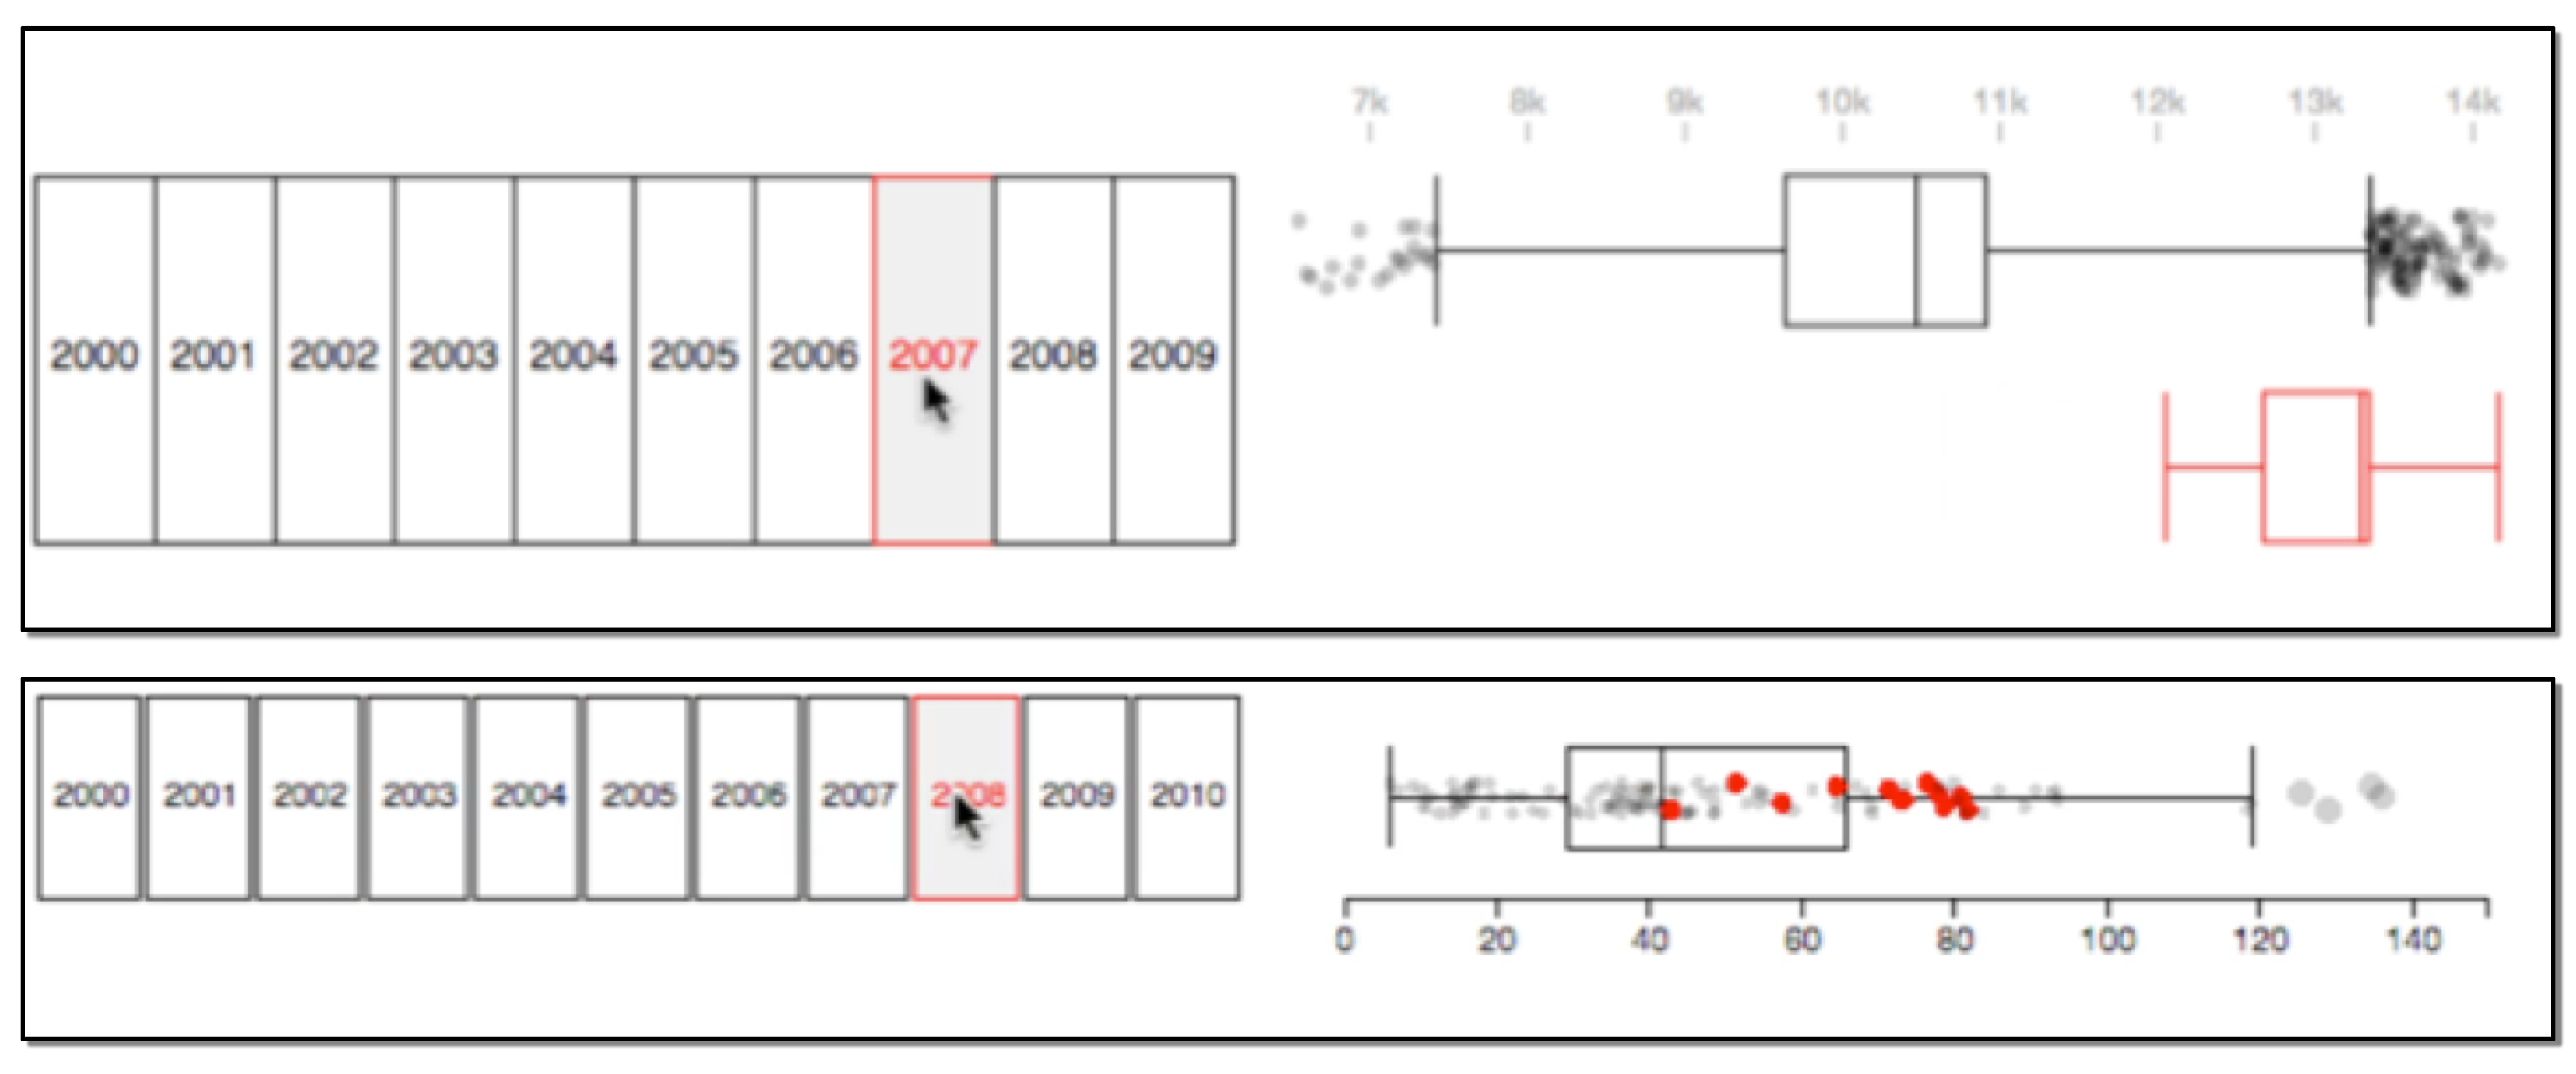
\includegraphics[width=0.95\columnwidth]{figures/d3-boxplots.pdf}}
	\vspace{-0.15cm}
	\caption{An interactive auxiliary boxplot prototype: boxplots corresponding to the brushed time period are shown alongside the boxplot for the entire time series.}
	\label{fig:interactive-boxplots}
	\vspace{-0.3cm}
\end{figure}

\bstart{Juxtaposed stack and facets} Another reason to juxtapose views is to support fast alternation between tasks.
Recall that the Drill Down ({\bf T2}) and Roll Up ({\bf T3}) tasks are often performed in alternation, and we were concerned about the loss of context when switching between stacked bar or area charts and faceted bar or line charts.
To prevent this loss of context, we juxtaposed the stacked chart with the faceted charts, and provide linked highlighting between elements in the stack and those in the facets, as shown in Figure~\ref{fig:sandbox-stacks}; as a result, both the Drill Down and Roll Up tasks are supported in a single display.
Currently, four facets are shown in a row, with additional facets wrapping to subsequent rows, sorted in the same order as the elements in the stack.

\begin{figure}[ht!]
    \vspace{-0.3cm}
	\centering
	\fbox{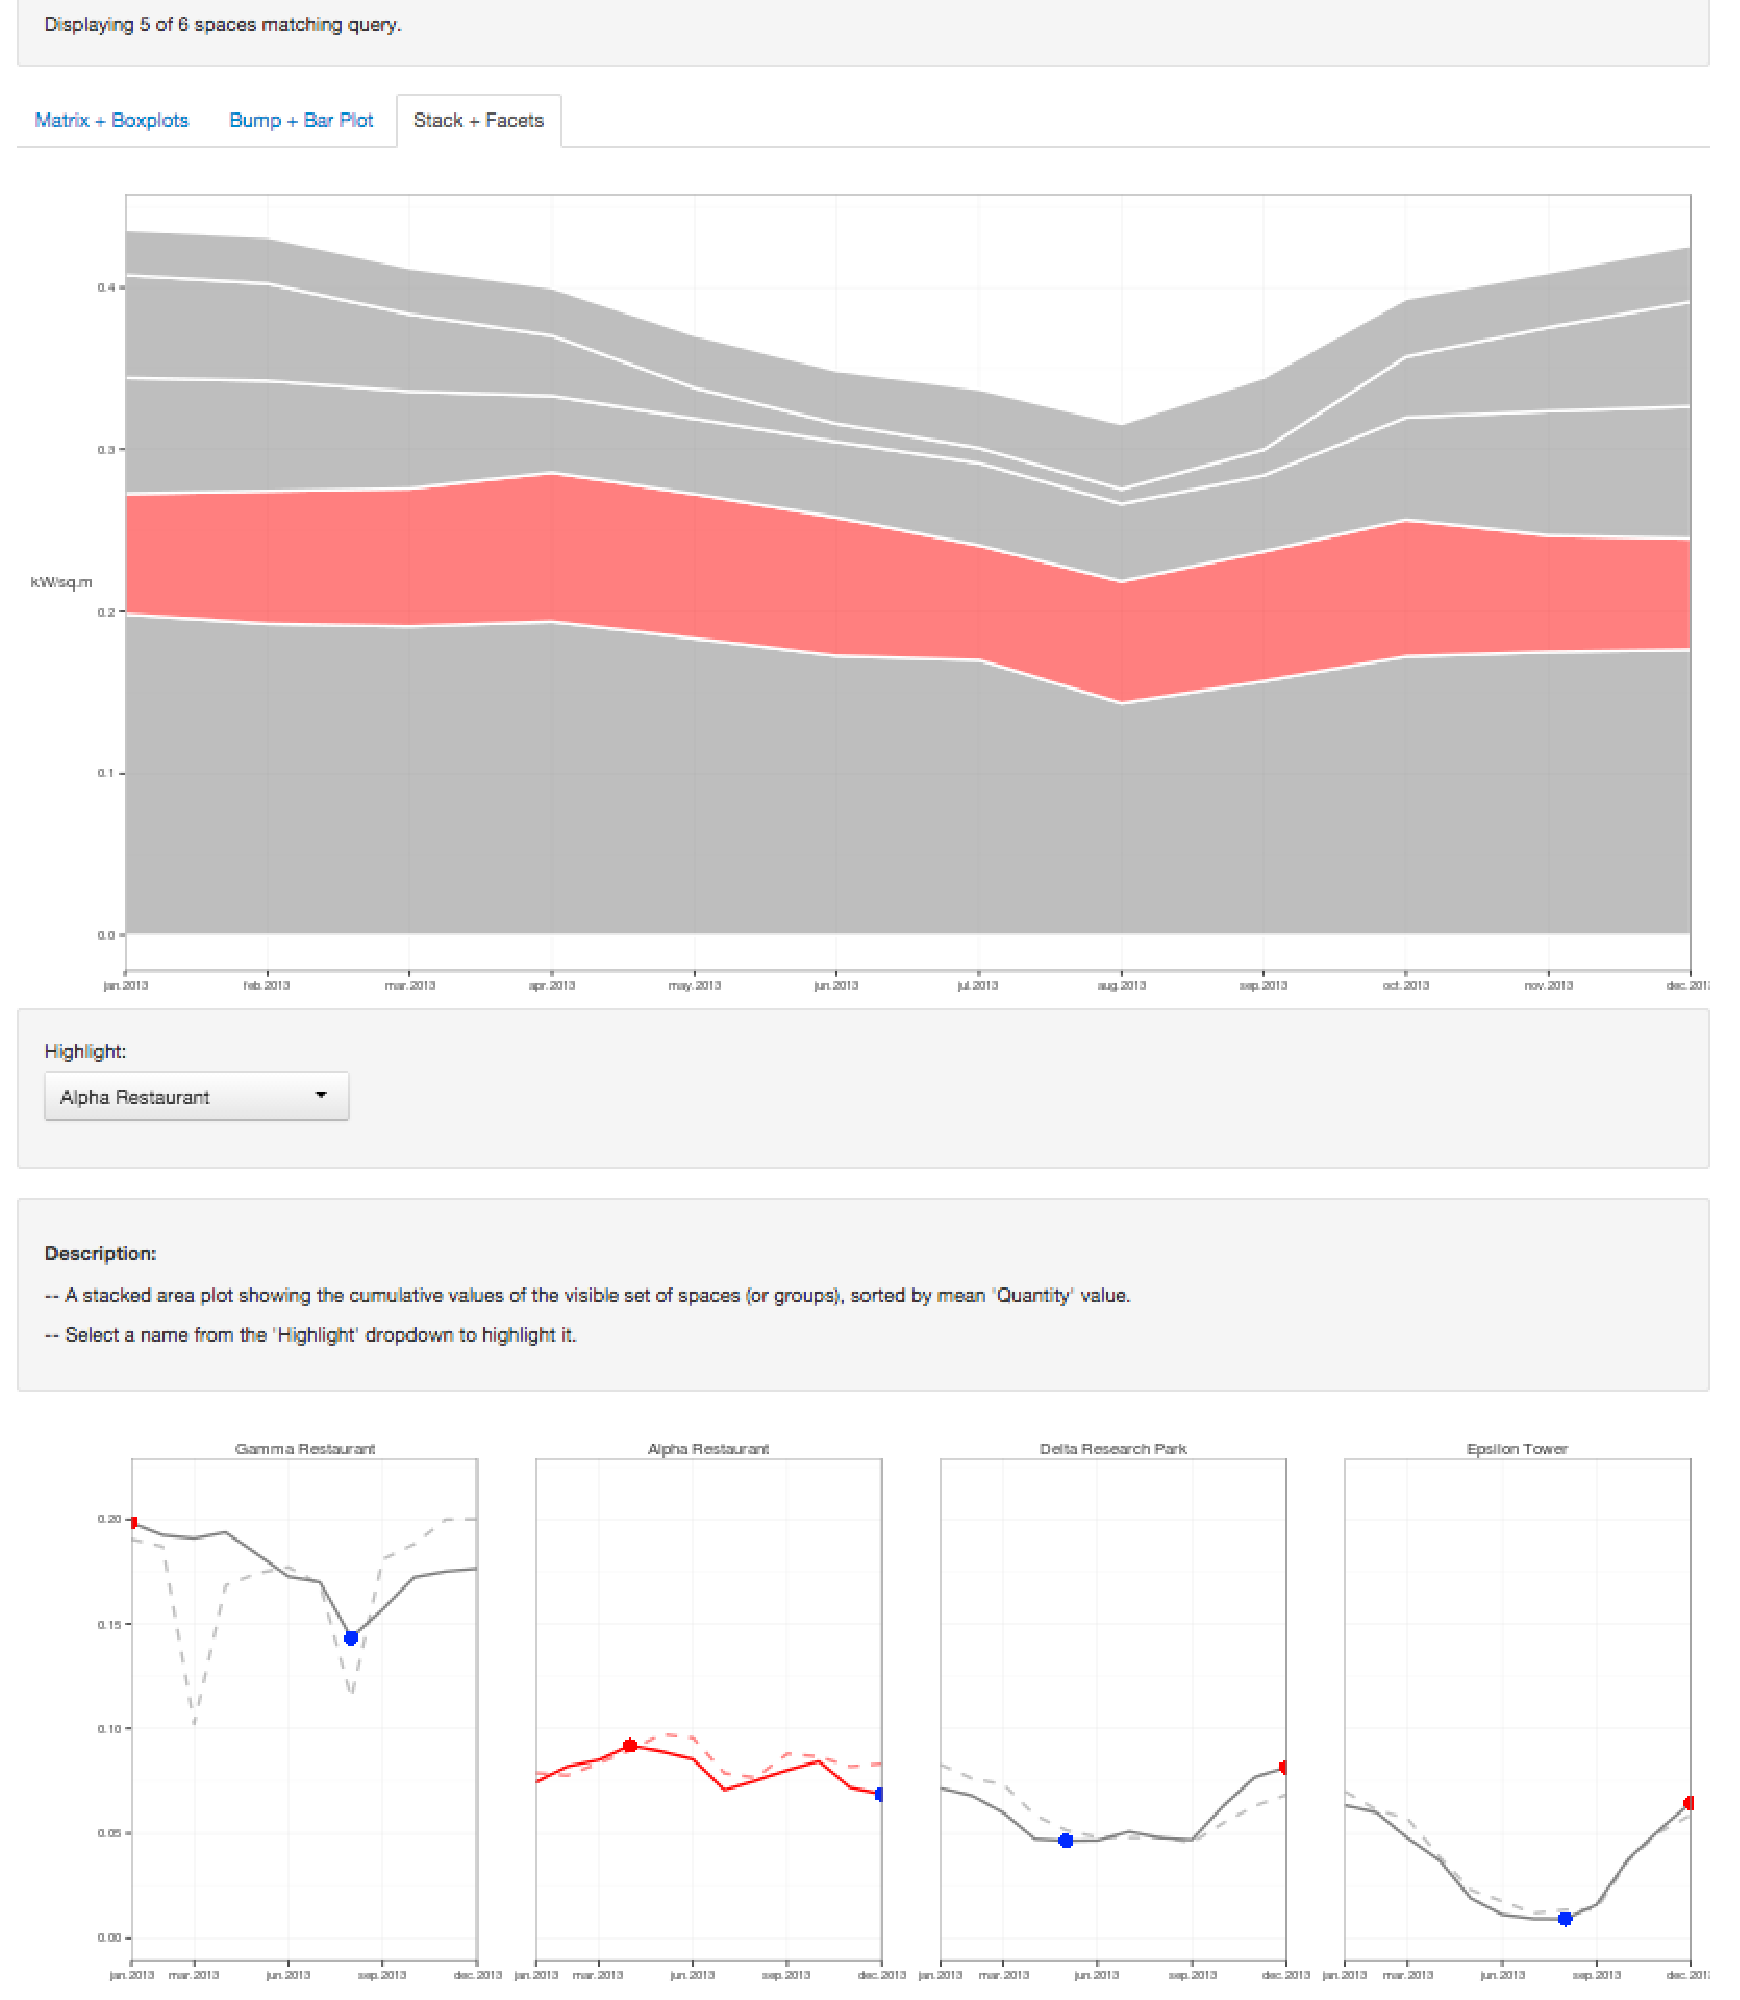
\includegraphics[width=0.95\columnwidth]{figures/sandbox-stacks.pdf}}
	\vspace{-0.15cm}
	\caption{A stacked area chart of \textsl{energy demand} data for 4 library buildings, juxtaposed alongside faceted line charts of the same data. The same building is highlighted in red in both the stack and the facets.}
	\label{fig:sandbox-stacks}
	\vspace{-0.3cm}
\end{figure}

\begin{figure*}[hbp!]
    \vspace{-0.3cm}
	\centering
	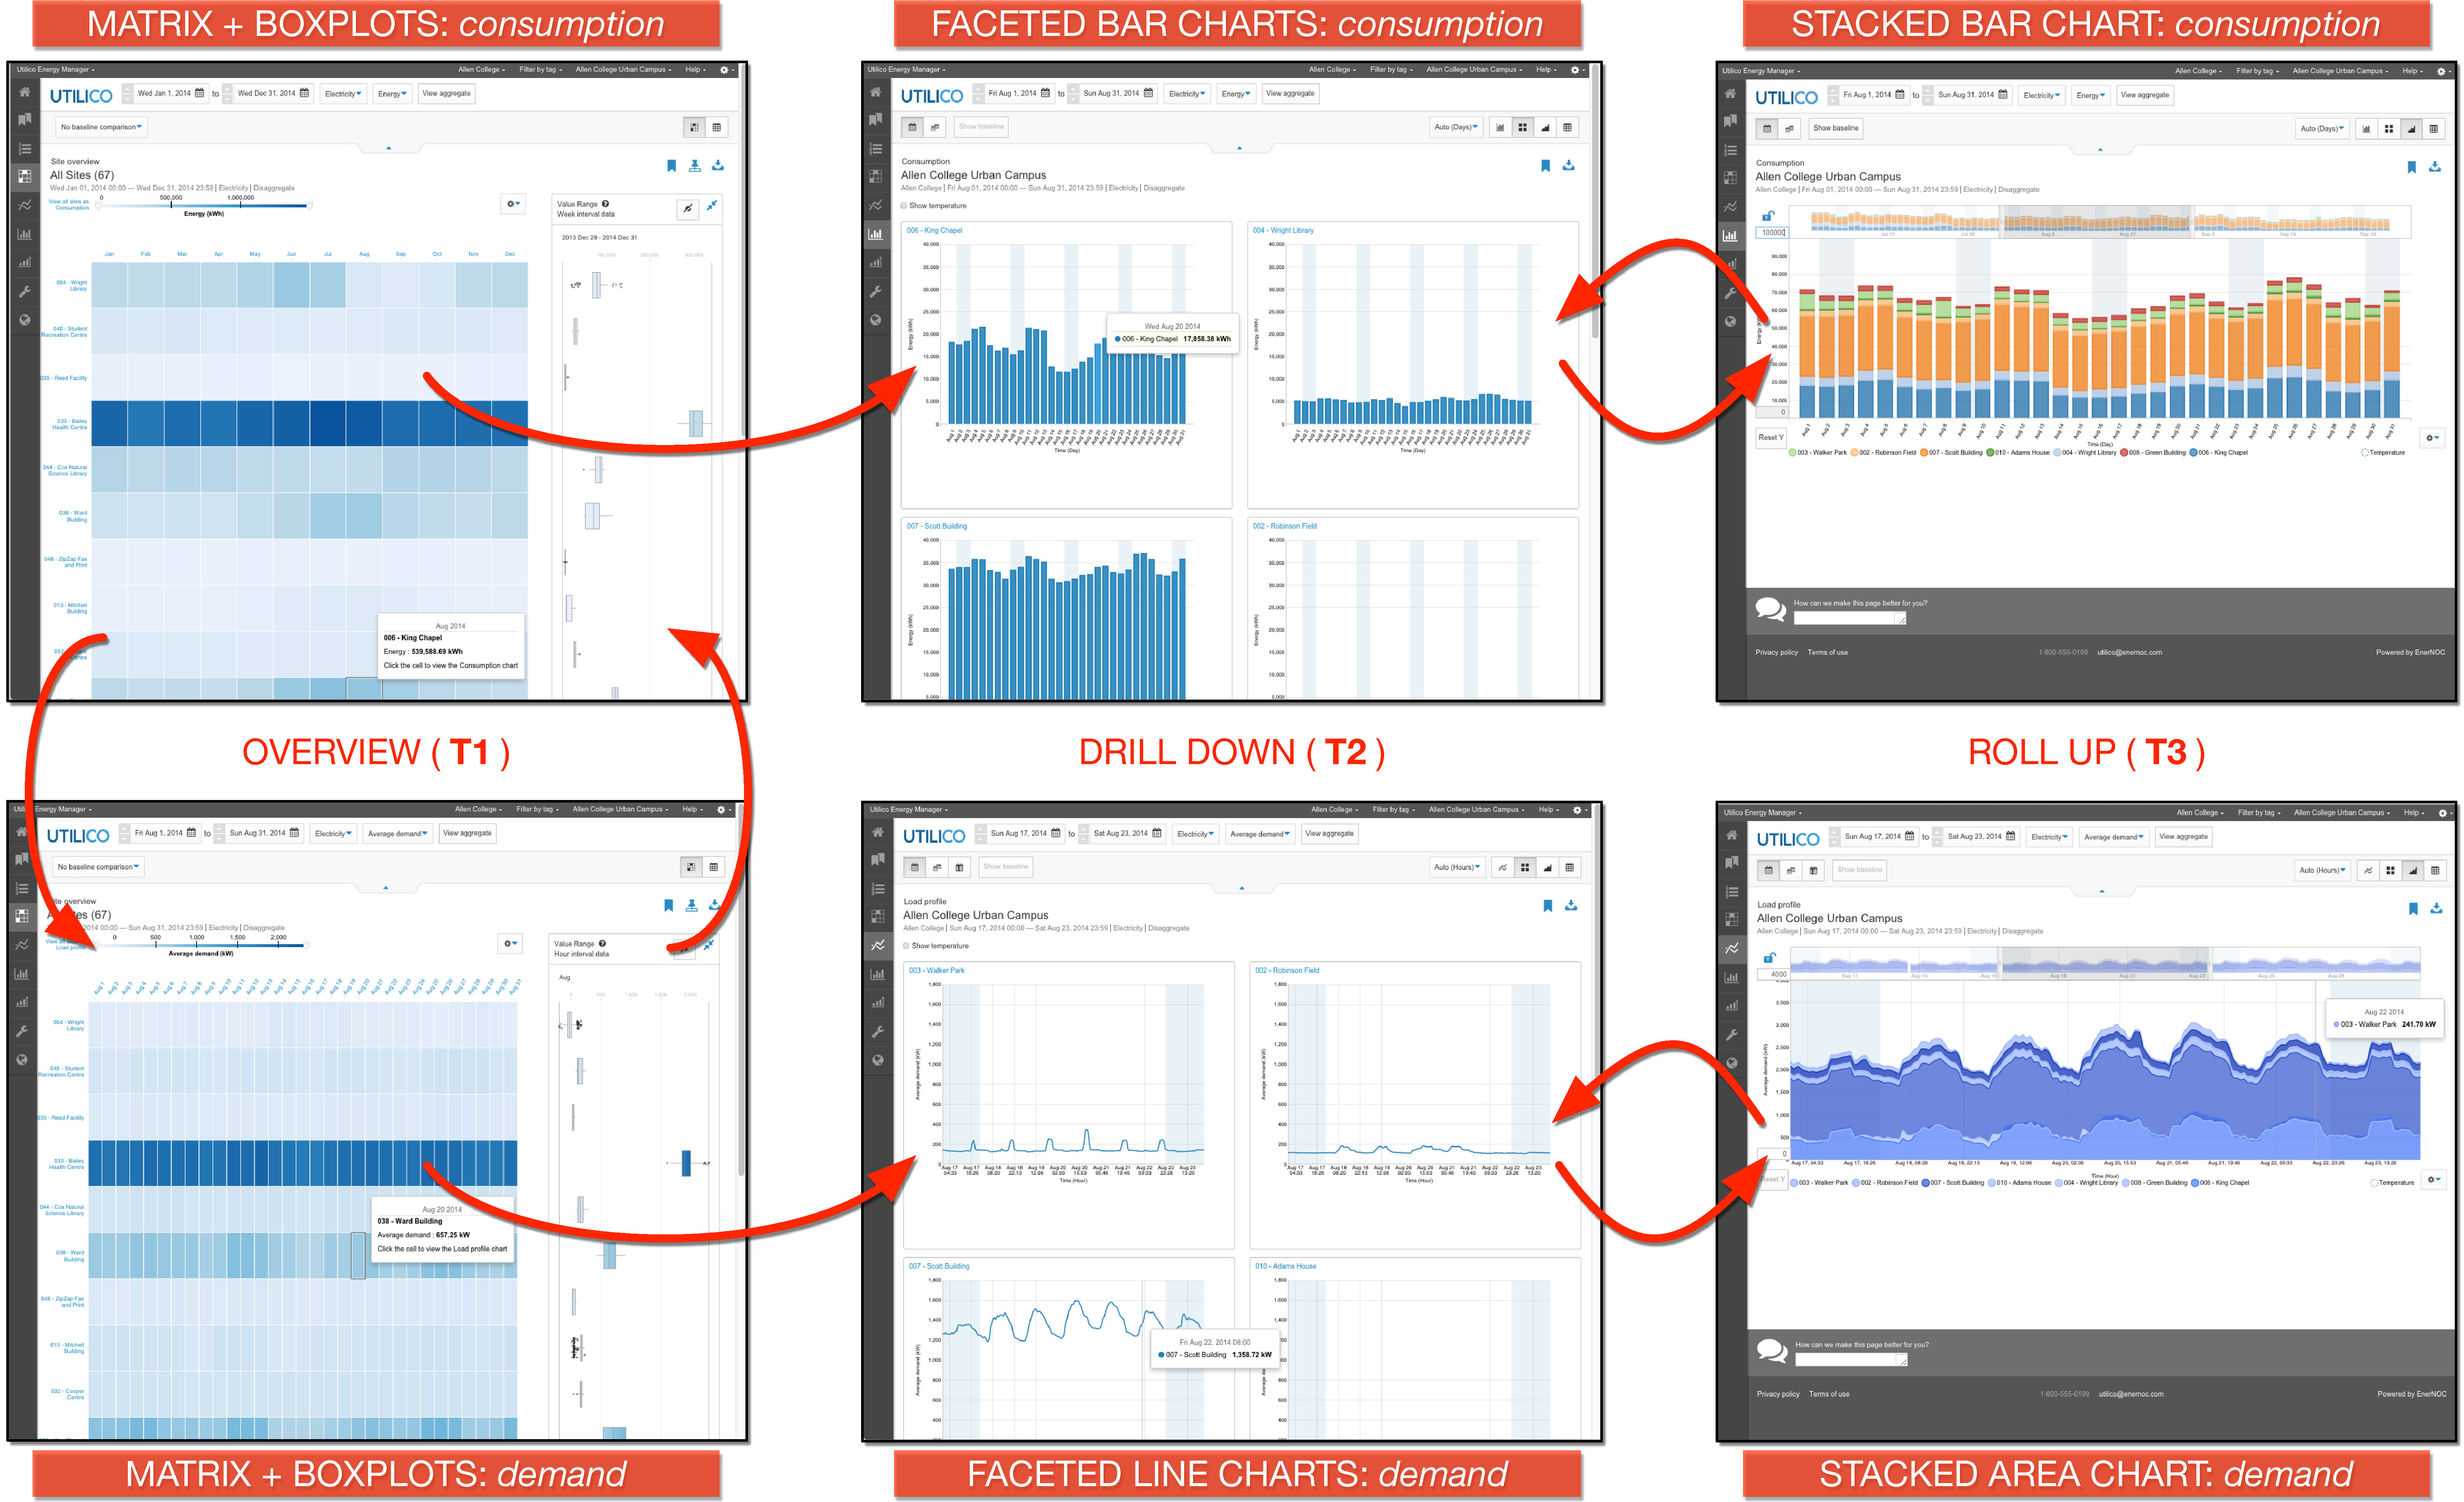
\includegraphics[width=0.975\textwidth]{figures/emu.pdf}
	\vspace{-0.3cm}
	\caption{The redesigned \textsl{Energy Manager} that incorporates many aspects of our prototype designs. On the left, the \textsl{Site Overview} (a time series matrix) is juxtaposed with coordinated \textsl{Value Range} (boxplot) views. An energy worker can easily switch between units such as \textsl{energy consumption} or \textsl{energy demand} and filter or aggregate the set of buildings to those that share a common categorical tag; by selecting a column of the matrix, she can drill down to faceted or stacked visualizations of \textsl{consumption} (top middle, top right) or \textsl{demand} (bottom middle, bottom right).}
	\label{fig:emu}
% 	\vspace{-0.6cm}
\end{figure*} 

\bstart{Sequenced view navigation}
% However, the sandbox did not allow us to directly investigate interactions involving coordinated selection across juxtaposed visualizations, nor did it allow us to easily prototype interactive workflows to support the task sequence 
Recall that the Drill Down ({\bf T2}) and Roll Up ({\bf T3}) tasks involve fewer buildings and finer temporal resolutions than the Overview ({\bf T1}) task, which has broader scope; 
thus, it would be inappropriate to juxtapose the Overview visualizations with the Drill Down and Roll Up visualizations in a single display.
Instead, we considered how an energy worker would navigate between these views shown on separate displays.
Beginning with the matrix and auxiliary boxplots, the energy worker can perform the Overview task, select units of interest, and filter or aggregate buildings in the portfolio. 
If the currently selected unit of interest is {\it consumption} or {\it intensity}, selecting a column of the matrix directs the energy worker to juxtaposed faceted and stacked bar charts that include every building from the matrix and spanning the time period corresponding to the selected column. 
For {\it demand} data, the energy worker is directed to faceted and stacked line charts.
At this point, the energy worker can perform the Drill Down and Roll Up tasks in alternation.
We demonstrate this multiple-view workflow in the supplemental video.

Finally, we also envisioned drilling down further to individual buildings. 
If the energy worker selects a cell or row of the matrix, she will navigate to a single bar or line chart for the corresponding building and time period.
% This workflow design, along with our consolidated findings from the feedback sessions, were presented to our collaborators to help them decide whether they should incorporate our designs into production development, and in which priority.
% \tm{the idea of workflows isn't front and center enough here yet, even though we use it below in table 4 line 4 to refer to this stuff.}


%-------------------------------------------------------------------------
%-------------------------------------------------------------------------

\section{Results}
\label{results}

%-------------------------------------------------------------------------
%-------------------------------------------------------------------------

We are pleased to report that our collaborators adopted a number of our visualization designs into a new version of Energy Manager, shown in Figure~\ref{fig:emu}, which will soon be deployed to their large client base.
Their client base is also expected to grow dramatically as a result of their recent partnership with a large utility company: tens of thousands of energy workers will now be able to analyze the energy performance of their building portfolios with the redesigned Energy Manager. 
% The size of portfolios will also grow, from hundreds to thousands of buildings.
% \mb{How many?} 
% \jn{Not sure about the number of new energy workers but maybe worth mentioning here that the portfolio sizes are also expected to dramatically increase in size, which the new Energy manager would now be able to better support.  For example, The Environment Agency for British Gas will have approximately 2000 "sites" or spaces a lot of them are pump stations.}

As in our sandbox environment, options for filtering and aggregating buildings according to shared categorical tags are now prominently and persistently shown in the menu at the top of the interface. 
% \jn{heavy importance on this from these new super large portfolios we are expecting.}
The interface also provides the ability to select units of interest and compare observed energy values against trusted historical values, as an alternative to comparing observed values to less trusted predicted values, overcoming a limitation of the original Energy Manager.

\bstart{Coordinated matrix and boxplots} a variant of our design described in Section~\ref{design:workflows} has been incorporated into the redesigned Energy Manager.
%; the matrix is labeled as a {\it Site Overview} to avoid the {\it heat map} misnomer, and corresponds well with our characterization of the Overview ({\bf T1}) task. 
% \jn{Internal debates still over what to call this, we might go back to Heatmap as that's the name of what the visualization is (Kevin's thoughts) doubts from Ben and I as to that for there reasons you've specified, just "Overview" was suggested.  User testing in the last 2 rounds showed confusion when Site Ranking and Site Overview are in the same menu, terms seem interchangeable, although things always change so not sure if it's worth mentioning here.}
% As in our sandbox, the buildings are shown in rank order according to the currently selected unit of interest. 
The number of buildings shown depends on the window size, and more buildings appear as the energy worker scrolls.
% Our collaborators also added the ability to interactively adjust the colour scale bounds of the matrix.
Our collaborators did consider the alternative calendar-based encoding, but ruled it out based on a requirement that arose late in the design process: that the redesigned Energy Manager be accessible on a tablet device. 
Partitioning the matrix cells into calendars may result in calendar dates too small to be selectable without zooming, which may incur a high implementation cost.
Meanwhile, the boxplots update when the energy worker brushes the matrix by hovering over a cell in the corresponding matrix row, similar to the behaviour of the prototype we described in Section~\ref{design:workflows}. 
Unlike our earlier prototype, a single boxplot is shown instead of showing one boxplot for the entire range and another boxplot for the brushed time period; when no time period in the matrix is brushed, the boxplot for the entire time series is shown.

\bstart{Interactive workflows realized} Another critical improvement over the original Energy Manager is the ability for an energy worker to drill down from a row, column, or cell of the matrix to stacked, faceted, superimposed, or individual line and bar charts, as shown in Figure~\ref{fig:emu}.
The selected energy unit is retained across these transitions, so faceted line charts and stacked area charts are used for {\it demand}, while faceted bar charts and stacked bar charts are used for {\it consumption}.
In faceted views, individual facets can be manually resorted via drag and drop.
Stacked and faceted visualizations are currently shown separately; our collaborators are considering juxtaposing stacked and faceted visualizations, such as in the design described in Section~\ref{design:workflows}, which would allow for an uninterrupted alternation between the Drill Down ({\bf T2}) and Roll Up ({\bf T3}) tasks in the same display.

%-------------------------------------------------------------------------
%-------------------------------------------------------------------------

\section{Discussion}
\label{discussion}

%-------------------------------------------------------------------------
%-------------------------------------------------------------------------

We now step back from specific aspects of visualization design for time-oriented data to discuss higher-level guidelines, to reflect upon on our methodology, and to suggest future work.

%-------------------------------------------------------------------------

\subsection{Guidelines: Familiarity and Trust}
\label{discussion-guidelines}

%-------------------------------------------------------------------------

In addition to the specific guidelines regarding matches and mismatches between idioms and abstractions described in Section~\ref{design:visenc}, we also propose more general and succinct guidelines relating to the themes of {\it familiarity} and {\it trust}.

\bstart{Familiarity} As with professionals in many other domains, energy workers are accustomed to working predominantly with familiar visual encodings, namely bars and lines.
When we introduced them to unfamiliar visualization designs, we learned several things:

{\it Persevere despite unfamiliarity}: Though counter-intuitive, we learned that the juxtaposition of a matrix and a boxplot, two unfamiliar encodings, together with coordinated interaction and highlighting, received more positive feedback than either of these encodings in isolation.
The issue of unfamiliarity with the time-series matrix was also partially resolved when we partitioned the cells into calendars.
We similarly persevered with the unfamiliar bump plot: by superimposing a layer of familiar bars on top of the bump plot, energy workers were able to more easily interpret this rank-based visualization.
% Similarly, energy workers indicated that the more complex diverging colour scales for derived {\it savings} values in the matrix were easier to interpret than the simpler unidirectional colour scales for observed energy values. %, or how providing the ability to adjust the colour scale bounds improved matrix interpretation. 
% We can experiment with introducing unfamiliar visual encoding elements via animation~\cite{Ruchikachorn2015}.

% add heatmap to calendar point

% {\it Combine familiar idioms}: Familiar visual encodings can be combined in unfamiliar ways, such as the bars and lines in the {\it bump + bar plot} of Section~\ref{design-ranking}. In this instance, the novel combination of familiar encodings was easily interpreted and energy workers responded enthusiastically to them. 
% We encourage others to try and report on other novel combinations of familiar idioms.

{\it Beware assuming familiarity}: Introducing visual idioms using names that are well-known in the visualization literature can be misleading when they allude to familiar concepts in a way that is unfamiliar to the target audience, as we found with energy workers and the word ``{\it heat map}''~\cite{Field2015,Wilkinson2009}.
We initially referred to the time-series matrices as ``heat maps'', but this visualization term led to considerable confusion because of conflicting domain conventions with the energy-related meaning of {\it heat} and expectations raised by the word {\it map}: this encoding does not show energy solely used for heating, nor does it show the geographic location of buildings\footnote{This confusion is not unique to the energy domain~\cite{Field2015,Wilkinson2009}.}. 
In the redesigned Energy Manager, the time-series matrix is referred to as a {\it Site Overview}.

We also had a difficult experience gathering feedback about boxplots because the name itself was unfamiliar. 
In the redesigned Energy Manager, the boxplots are referred to as the {\it Value Range} visualization, a term that appears to be understood. % move the stuff from previous results section to here
In hindsight, we could have explicitly solicited visualization names from energy workers early on in the process based on their own descriptions~\cite{Metoyer2012}. 

\bstart{Trust} When visualization is used as part of the hypothesis generation and verification process, trust is imperative, especially for derived and aggregated values. %\jn{read a bit strange to me, added "a"}.
Previous work has investigated the trustworthiness of visualizations for text-based data~\cite{Chuang2012}, and we now discuss the topic of trust motivated by our design of visualizations of time-oriented data.

{\it Auxiliary charts to combat information loss}: When the number of concurrent time series grows large, it is difficult and overwhelming to visualize individual values from each time series; instead, a common approach is to visualize derived aggregate values~\cite{McLachlan2008}.
This loss of detail is apparent in the original Energy Manager's portfolio dashboard (Figure~\ref{fig:energy-manager}a) as well as in the cells of our time series matrix (Figure~\ref{fig:sandbox}).
Whenever there is a loss of detail, there is a loss of trust: one of the power user energy workers remarked that these derived aggregate values hide information such as extreme values.
In juxtaposing the time series matrix with auxiliary boxplots that update whenever a matrix cell containing an aggregate value is brushed, we are not only restoring lost information: we are also restoring trust.

{\it Promote agency over derived values}: In our sandbox environment and in the redesigned Energy Manager, we provided explicit and obvious interactive controls for filtering, aggregation, normalization, and unit selection, controls that were missing in the original Energy Manager.
With these controls, we provide energy workers agency over the creation of derived values and these values become more trusted.
Similarly, the redesigned Energy Manager includes the option to compare observed energy performance to selected historical values, as an alternative to comparing against predicted values generated by a ``black box'' statistical model; until there is some visual indication as to how the underlying model algorithms generate these values~\cite{Muhlbacher2014}, there will be little trust, and it is therefore preferable to provide the option to compare against trusted historical values.

%-------------------------------------------------------------------------

\subsection{Methodological Reflection}
\label{discussion-methodology}

%-------------------------------------------------------------------------

% We employed several methods and generated multiple research artefacts at each phase of this project.
% , as indicated in Table~\ref{tab:methodology}.
Though our overall methodological approach is similar to many other visualization design studies~\cite{McKenna2014,Sedlmair2012}, there are some specific aspects of our methodology that are unique to projects executed in company settings~\cite{Sedlmair2011}: we negotiated access to clients and to their portfolio data at the very beginning of our collaboration, and we encourage researchers considering similar collaborations to do the same.
In addition, we also engaged primarily with remote energy workers, and our methodological decisions described in Section~\ref{methodology} reflect this logistical difficulty~\cite{Brehmer2014a}.
We now take the opportunity to reflect on three other aspects of our methodology:

% \begin{table}[ht]\renewcommand{\arraystretch}{1}\addtolength{\tabcolsep}{-1pt}
%     \vspace{-.3cm}
%     \begin{center}
%     \scriptsize
%     \begin{tabular}{l|c|*{4}l}
    
%         \rowcolor{gray!15}
    
%         & & \multicolumn{4}{c}{\bf Artefacts}
        
%         \\

%         \rowcolor{gray!15}
    
%         {\bf Phase} & \rot{{\bf Duration} (months)} & \rot{slides, demos} & \rot{interviews} & \rot{annotations} & \rot{summary}
        
%         \\
        
%         \hline  
        
%         (i) Work domain analysis & 5 & & \OK & & \OK
        
%         \\
        
%         (ii) Define and verify abstractions & 1 & \OK & \OK & \OK & \OK
        
%         \\
        
%         (iii) Develop visualization sandbox & 4 & \OK & & & \OK
        
%         \\
        
%         (iv) Evaluate sandbox visualizations & 3 & \OK & \OK & \OK & \OK
        
%         \\
        
%         (v) Prototyping interactions, workflows & 6 & \OK & & & 
        
%         \\
        
%         (vi) Production by collaborator & 12+ & \OK & \OK & \OK &
        
%         \\
        
%     \end{tabular}
%     % \vspace{-0.3cm}
%     \caption{Phases of our methodology and associated research artefacts.}
%     \label{tab:methodology}
%     \end{center}
%     \vspace{-0.6cm}
% \end{table}

\bstart{Work domain analysis} {\it Worth it, and don't be daunted}. 
Conducting a rigorous and systematic work domain analysis can be time consuming and logistically challenging.
However, it is helpful to realize that authorities on work domain analysis~\cite{Vicente1999} established their methodologies in the design of high-risk, high-cost systems, such as nuclear power plant control rooms.
Work domain analysis and requirements analysis methodologies for many visualization design projects can be more flexible~\cite{McNamara2014} and creative~\cite{Goodwin2013}.
A thorough work domain analysis need not take a year to complete, and subsequent phases of abstraction and iterative design can be carried out while continuing to develop an understanding of the work domain.

\bstart{Workflow prototyping} 
In addition to using our sandbox environment to identify appropriate visual encodings for individual tasks, we also used it as a tool to generate possible {\it workflows} that support a sequence of tasks.
Some visualization research projects stop before this step, but we argue for its importance.
We thought that confronting energy workers with a combinatorial explosion of possibilities from a large set of visual encodings and view parametrization options would fall short of a full solution to the problem at hand.

% \bstart{Stakeholder complexity} {\it Negotiate relationships early}.  
% Sedlmair~\etal~\cite{Sedlmair2011} discussed methodological considerations for visualization design and evaluation in corporate settings, and we certainly faced many of the challenges that they identified. 
% % Many visualization design collaborations between academic researchers and companies involve designing for the company's {\it employees}, whereas we encountered an additional degree of separation in that we were designing for the collaborator's {\it clients}.

\bstart{Grounding design decisions} {\it Document everything, strive to be consistent and systematic}. 
One collaborator remarked that our approach often confirmed some earlier suspicions rather than introduced major surprises, where the novelty lay in a clear path to design decision-making that was missing before: {\it ``we performed an analysis of} [{\it Energy Manager's}] {\it flaws in a systematic way, put a name on them, and then tested with users''}. 
% \tm{tried to punch this up a bit to be more clear, think still needs more work}
The exhaustive collecting and analyzing of qualitative data before and during design allowed us to justify the design decisions described in Sections~\ref{design:visenc} and~\ref{design:workflows}. 
Presenting our consolidated findings and design justifications in concise and consistent annotated slide decks was highly appreciated by our collaborators.
Given this presentation of evidence, our collaborators adopted our designs with confidence, much in the same way that the results of a controlled quantitative experiment can convince stakeholders~\cite{Sedlmair2011}. 

%-------------------------------------------------------------------------

\subsection{Future Work}
\label{discussion-future-work}

%-------------------------------------------------------------------------

This paper focused on the visualization design and evaluation process and how our designs were adopted into our collaborators' production timeline.
In the future, we would like to assess the adoption of the redesigned Energy Manager following its wide-scale deployment in Summer 2015. 
We will track usage over an extended period of time and speak to more energy workers via interviews and focus groups.

%-------------------------------------------------------------------------
%-------------------------------------------------------------------------

\section{Conclusion}
\label{conclusion}

%-------------------------------------------------------------------------
%-------------------------------------------------------------------------

We conducted a design study in the energy domain, one in which we collaborated with an energy analysis software company and their clients to develop visualizations for analyzing the energy performance of large building portfolios.
We described generalizable visualization design choices framed in terms of {\bf matches} and {\bf mismatches} between abstractions and visual encoding idioms that are transferable beyond the energy analysis domain.
We also contributed more general guidelines pertaining to the themes of {\bf familiarity} and {\bf trust}, along with {\bf methodological guidance} for visualization design studies. % and considerations for projects with industry collaborators.
As a result of our research and design process, our visualization designs were adopted by our collaborator into their development of a redesigned commercial energy analysis application that will be deployed to tens of thousands of energy workers.

%%%%%%%%%%%%%%%%%%%%%%%%%%%%%%%%%%%%%%%%%%%%%%%%%%%%%%%%%%%%%%%%
%%%%%%%%%%%%%%%%%%%%%% END OF THE PAPER %%%%%%%%%%%%%%%%%%%%%%
%%%%%%%%%%%%%%%%%%%%%%%%%%%%%%%%%%%%%%%%%%%%%%%%%%%%%%%%%%%%%%%%%

%% if specified like this the section will be committed in review mode
\acknowledgments{
We received financial support from NSERC and Mitacs. 
We thank our collaborators at EnerNOC, including client services liaison J. Christopherson, as well as C. Crane and the Energy Manager development team.
We also thank the energy workers that we interviewed. 
Thanks to M. Borkin, A. Cri\c{s}an, J. Dawson, J. Fulda, E. Hoque, S.-H. Kim, N. Mahyar, J. McGrenere, and the anonymous reviewers for their feedback on the paper. 
% \tm{should enamul hoque be in here, or was he not at any of these sessions?}
}

\bibliographystyle{abbrv}
%%use following if all content of bibtex file should be shown
%\nocite{*}
\bibliography{emu-infovis15}
\end{document}
